% Options for packages loaded elsewhere
\PassOptionsToPackage{unicode}{hyperref}
\PassOptionsToPackage{hyphens}{url}
\PassOptionsToPackage{dvipsnames,svgnames*,x11names*}{xcolor}
%
\documentclass[
]{article}
\usepackage{lmodern}
\usepackage{amsmath}
\usepackage{ifxetex,ifluatex}
\ifnum 0\ifxetex 1\fi\ifluatex 1\fi=0 % if pdftex
  \usepackage[T1]{fontenc}
  \usepackage[utf8]{inputenc}
  \usepackage{textcomp} % provide euro and other symbols
  \usepackage{amssymb}
\else % if luatex or xetex
  \usepackage{unicode-math}
  \defaultfontfeatures{Scale=MatchLowercase}
  \defaultfontfeatures[\rmfamily]{Ligatures=TeX,Scale=1}
  \setmainfont[]{lm}
\fi
% Use upquote if available, for straight quotes in verbatim environments
\IfFileExists{upquote.sty}{\usepackage{upquote}}{}
\IfFileExists{microtype.sty}{% use microtype if available
  \usepackage[]{microtype}
  \UseMicrotypeSet[protrusion]{basicmath} % disable protrusion for tt fonts
}{}
\makeatletter
\@ifundefined{KOMAClassName}{% if non-KOMA class
  \IfFileExists{parskip.sty}{%
    \usepackage{parskip}
  }{% else
    \setlength{\parindent}{0pt}
    \setlength{\parskip}{6pt plus 2pt minus 1pt}}
}{% if KOMA class
  \KOMAoptions{parskip=half}}
\makeatother
\usepackage{xcolor}
\IfFileExists{xurl.sty}{\usepackage{xurl}}{} % add URL line breaks if available
\IfFileExists{bookmark.sty}{\usepackage{bookmark}}{\usepackage{hyperref}}
\hypersetup{
  pdftitle={Adoption of Climate-Resilient Groundnut Varieties Increases Agricultural Production, Consumption, and Smallholder Commercialization in West Africa},
  pdfauthor={Martin Paul Jr.~Tabe-Ojong, Jourdain Lokossou, Bisrat Gebrekidan, Hippolyte D. Affognon},
  colorlinks=true,
  linkcolor=Maroon,
  filecolor=Maroon,
  citecolor=Blue,
  urlcolor=Blue,
  pdfcreator={LaTeX via pandoc}}
\urlstyle{same} % disable monospaced font for URLs
\usepackage{longtable,booktabs}
\usepackage{calc} % for calculating minipage widths
% Correct order of tables after \paragraph or \subparagraph
\usepackage{etoolbox}
\makeatletter
\patchcmd\longtable{\par}{\if@noskipsec\mbox{}\fi\par}{}{}
\makeatother
% Allow footnotes in longtable head/foot
\IfFileExists{footnotehyper.sty}{\usepackage{footnotehyper}}{\usepackage{footnote}}
\makesavenoteenv{longtable}
\setlength{\emergencystretch}{3em} % prevent overfull lines
\providecommand{\tightlist}{%
  \setlength{\itemsep}{0pt}\setlength{\parskip}{0pt}}
\setcounter{secnumdepth}{5}
\usepackage[margin=2.8cm]{geometry}
\renewcommand{\contentsname}{Table of Contents}
\usepackage{enumitem}
\usepackage{pifont}
\renewcommand{\labelitemi}{$\rightarrow$}
\usepackage{tocloft}
\renewcommand\cftsecleader{\cftdotfill{\cftdotsep}}
\usepackage{hyperref}
\hypersetup{linkcolor = blue}
\usepackage{hanging}
\usepackage[T1]{fontenc}
\usepackage{graphicx}
\usepackage{booktabs,threeparttablex}
\usepackage{pdflscape}
\usepackage{fvextra}
\DefineVerbatimEnvironment{Highlighting}{Verbatim}{breaklines,commandchars=\\\{\}}
\usepackage{pdfpages}
\usepackage{fouriernc}
\usepackage{caption}
\usepackage{nimbusmono}
\renewcommand{\thetable}{S\arabic{table}}
\renewcommand{\thefigure}{S\arabic{figure}}
\setlength{\cfttabnumwidth}{1cm}
\usepackage{booktabs}
\usepackage{longtable}
\usepackage{array}
\usepackage{multirow}
\usepackage{wrapfig}
\usepackage{float}
\usepackage{colortbl}
\usepackage{pdflscape}
\usepackage{tabu}
\usepackage{threeparttable}
\usepackage{threeparttablex}
\usepackage[normalem]{ulem}
\usepackage{makecell}
\usepackage{xcolor}
\ifluatex
  \usepackage{selnolig}  % disable illegal ligatures
\fi

\title{Adoption of Climate-Resilient Groundnut Varieties Increases Agricultural Production, Consumption, and Smallholder Commercialization in West Africa}
\usepackage{etoolbox}
\makeatletter
\providecommand{\subtitle}[1]{% add subtitle to \maketitle
  \apptocmd{\@title}{\par {\large #1 \par}}{}{}
}
\makeatother
\subtitle{Supplementary Information}
    \usepackage{authblk}
              
            \author{Martin Paul Jr.~Tabe-Ojong, Jourdain Lokossou, Bisrat Gebrekidan, Hippolyte D. Affognon}
            \date{}

\begin{document}
\maketitle

\newpage
\tableofcontents
\newpage
\listoftables
\newpage

\newpage

\newpage

\hypertarget{supplementary-tables}{%
\section{Supplementary Tables}\label{supplementary-tables}}

\hypertarget{supplementary-note}{%
\subsection{Supplementary Note}\label{supplementary-note}}

We present the results of the estimation using the pooled FE-OLS model. Figure S1 presents the results of the relationship between the adoption of climate-resilient groundnut varieties and commercialization where we employ the linear probability model for binary outcomes. We present results when we consider adoption as a dummy and the extent of adoption of climate-resilient groundnut varieties. Considering adoption as a dummy, we establish a positive association with the commercialization outcomes; market participation, quantity of groundnut sold, and sales. Considering the area under adoption, we obtain negative estimates that are not statistically significant. However, this result could mean that increasing the area of cultivation of improved climate-resilient groundnut varieties is negatively correlated with market participation, quantity sold and the associated sales value. This negative relationship although not statistically significant could be due to diminishing returns when we consider the area under adoption. Otherwise, these negative results could be due to endogeneity issues which could lead to biased estimates. Given that we control for these endogeneity issues using the 2SLS and both household fixed effects and the correlated random effects model, we only use these results for comparison with the main estimation results.

\begin{figure}[htbp]
\centering
\caption{OLS estimates of the relationship between adoption and commercialization}
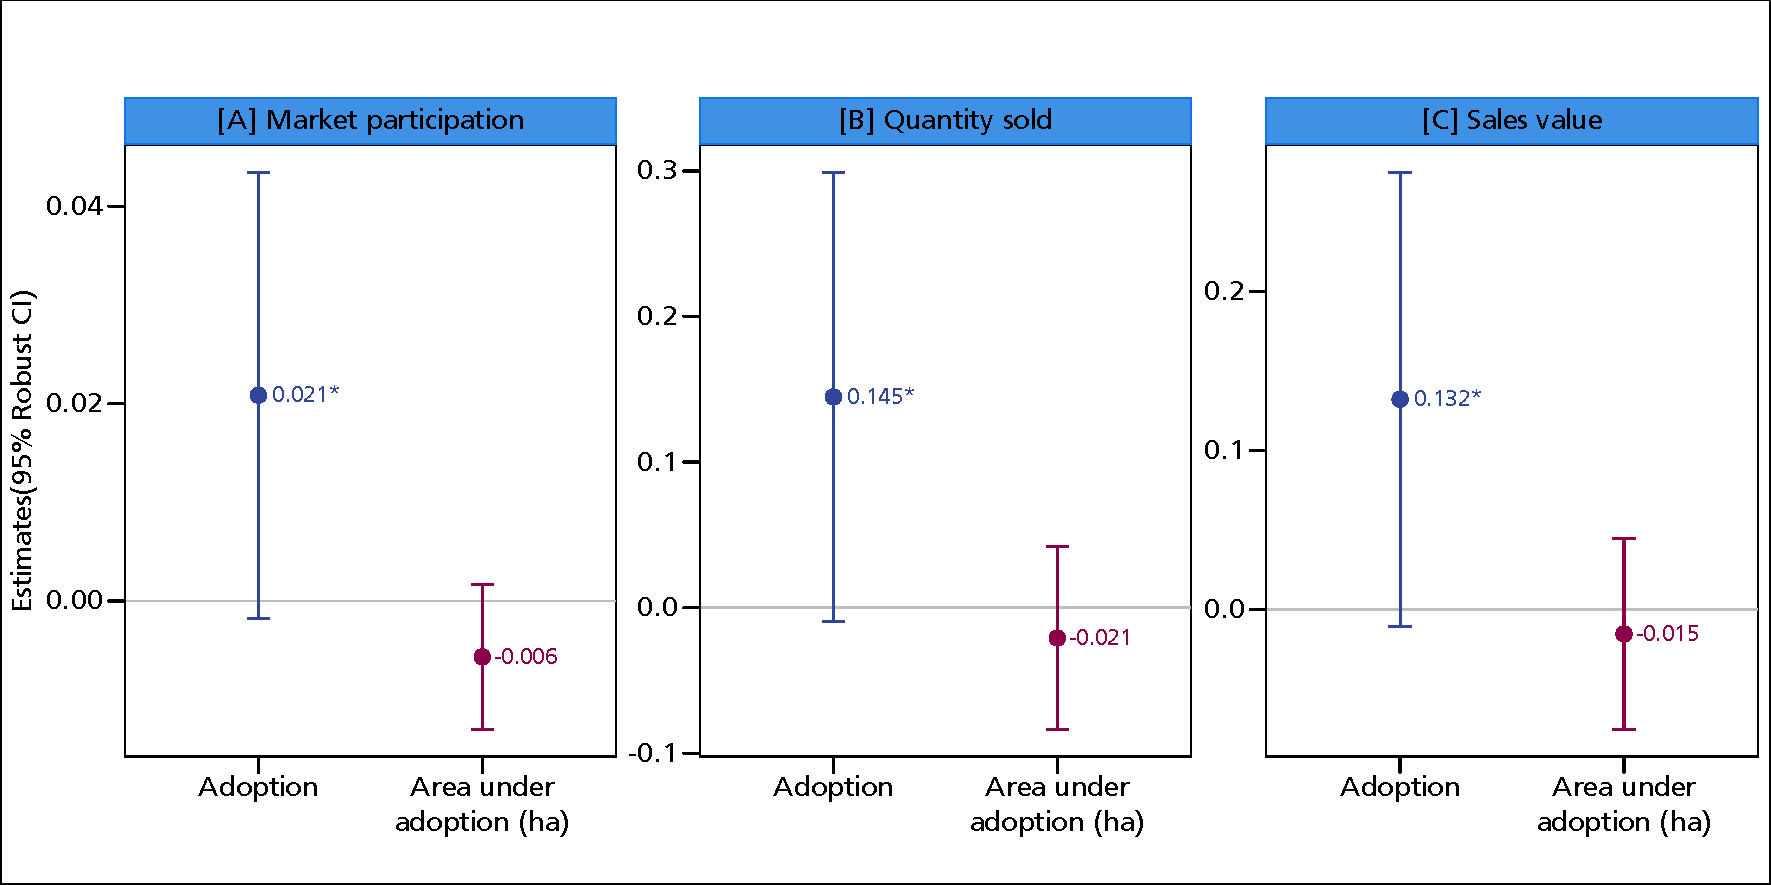
\includegraphics[width=\textwidth]{figures/fig_SM1.pdf}

\caption*{
Note: The graph displays coefficients along with their corresponding 95\% confidence intervals as error bars. The coefficents are estimated using OLS with n=8604 observation.The presence of an asterisk (*) above a coefficient indicates that the coefficient is statistically different from zero at a predetermined level of significance (*** p<0.01, ** p<0.05, * p<0.1).Statistical tests are two-sided t-tests. Full models are reported in S2 \& S3 with  Robust standard errors in parentheses and P-values in square brackets. Additional controls include age and educational level of the household head, dependency ratio, whether the household head is male, household size, cooperative membership, training, access to public and private extension, access to credits both in cash and kind, distance to nearest urban and village market, crop rotation, mixed cropping, labour, market price, input costs, area of cultivation, off-farm income and soil type.
}
\end{figure}
\newpage

Estimating the relationship between adoption of improved groundnuts, production, production value and land productivity using the FE-OLS model (Figure S2), we obtain positive coefficients for all outcomes. When we consider adoption as a dummy, we observe production and productivity increases of about 540Kg and 285Kg/ha respectively. Considering the scale of adoption, we observe that adoption of improved climate-smart groundnut varieties increases groundnut production by 240Kg and land productivity by approximately 60Kg/ha. The magnitudes here are positive indicating that adoption both when considered as a dummy as well as extent increases yield, production, and production value. The smaller magnitudes here might be indicative of diminishing returns as early highlighted. The positive and significant estimates of the area under adoption variable aligns with the tenets of the non-separable agricultural household model where the production, consumption and ultimately commercialization decisions of households are non-separable. This suggests that households would only participate in markets to the extent that the household food production and consumption needs are met.

\begin{figure}[htbp]
\centering
\caption{OLS estimates of the relationship between adoption and commercialization}
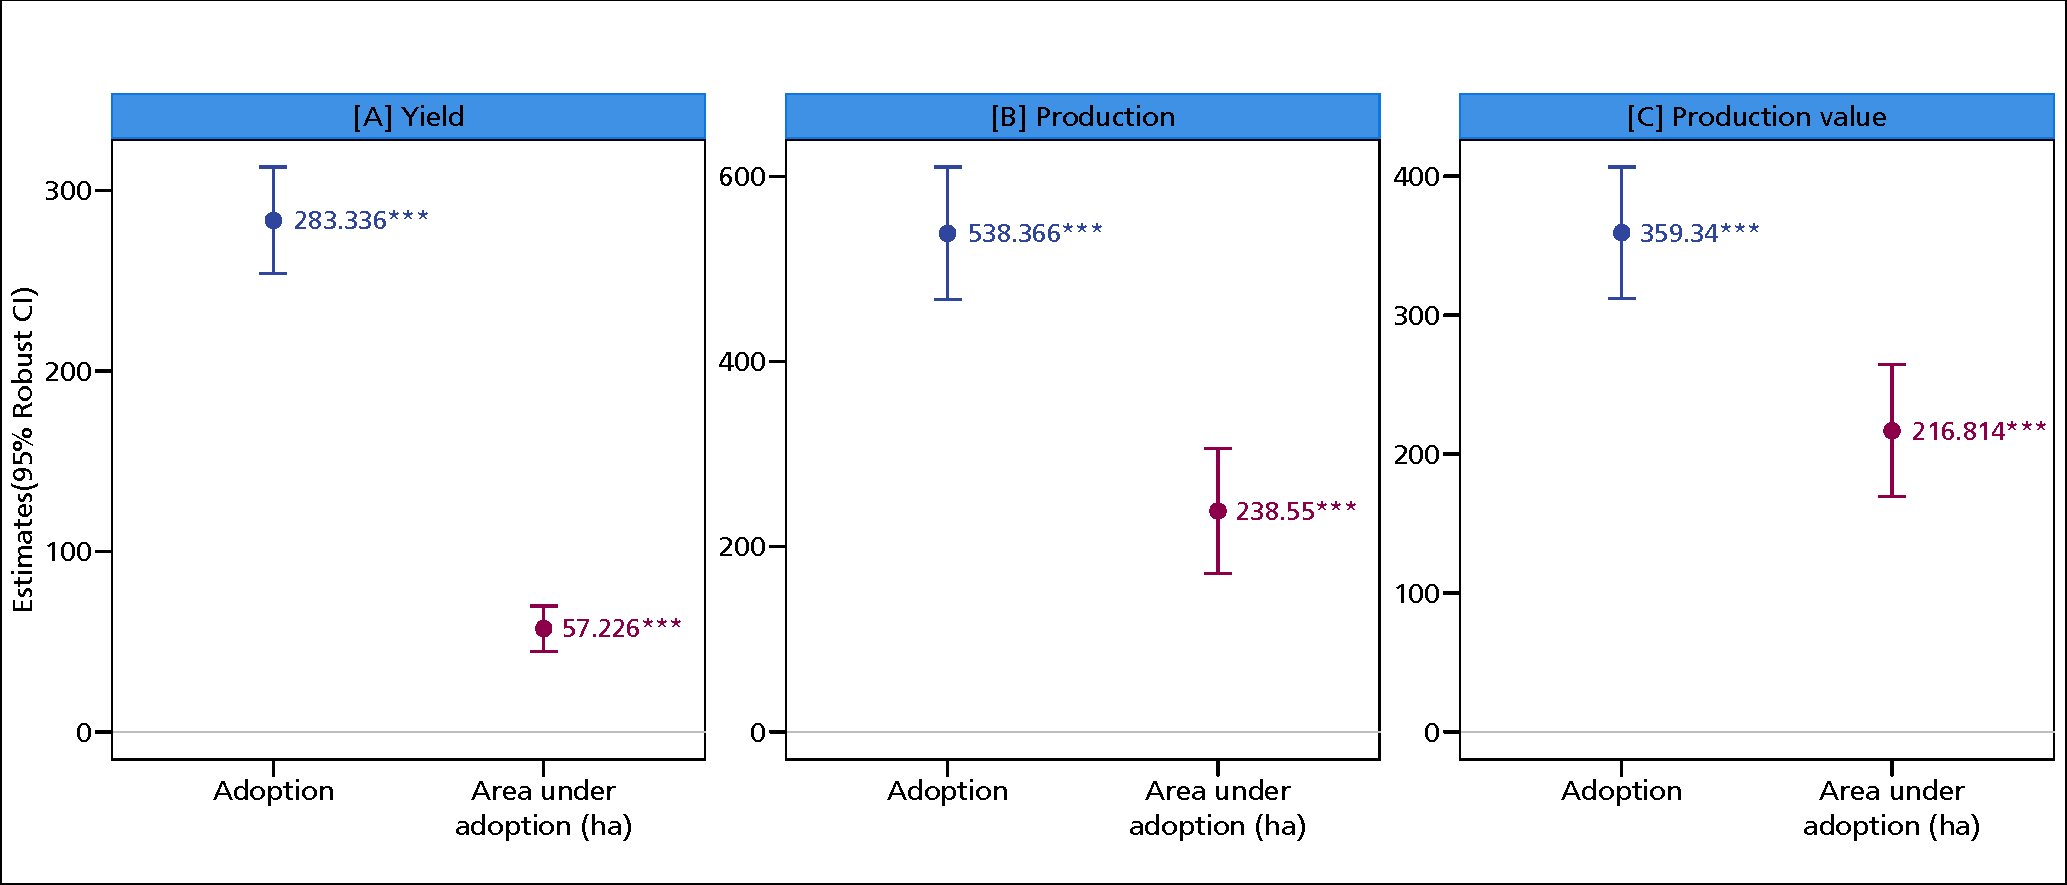
\includegraphics[width=\textwidth]{figures/fig_SM2.pdf}
\caption*{
Note: The graph displays coefficients along with their corresponding 95\% confidence intervals as error bars. The coefficents are estimated using OLS with n=8604 observation.The presence of an asterisk (*) above a coefficient indicates that the coefficient is statistically different from zero at a predetermined level of significance (*** p<0.01, ** p<0.05, * p<0.1). Statistical tests are two-sided t-tests. Full models are reported in S4 \& S5 with  Robust standard errors in parentheses and P-values in square brackets. Additional controls include age and educational level of the household head, dependency ratio, whether the household head is male, household size, cooperative membership, training, access to public and private extension, access to credits both in  cash and kind, distance to nearest urban and village market, crop rotation, mixed cropping, labour, market price, input costs, area of cultivation, off-farm income and soil type.
}
\end{figure}

\newpage

\hypertarget{descriptive-statistics}{%
\subsection{Descriptive statistics}\label{descriptive-statistics}}

\begin{landscape}\begin{table}[!h]

\caption{\label{tab:unnamed-chunk-2}Descriptive statistics by year and adoption status}
\centering
\resizebox{\linewidth}{!}{
\fontsize{6}{8}\selectfont
\begin{threeparttable}
\begin{tabular}[t]{lccccccccc}
\toprule
\multicolumn{1}{c}{ } & \multicolumn{3}{c}{\textbf{2017}, N = 2868} & \multicolumn{3}{c}{\textbf{2018}, N = 2868} & \multicolumn{3}{c}{\textbf{2019}, N = 2868} \\
\cmidrule(l{3pt}r{3pt}){2-4} \cmidrule(l{3pt}r{3pt}){5-7} \cmidrule(l{3pt}r{3pt}){8-10}
\textbf{Characteristic} & \textbf{Non-adopter}, N = 1,809 & \textbf{Adopter}, N = 1,059 & \textbf{p-value} & \textbf{Non-adopter}, N = 1,770 & \textbf{Adopter}, N = 1,098 & \textbf{p-value} & \textbf{Non-adopter}, N = 1,670 & \textbf{Adopter}, N = 1,198 & \textbf{p-value}\\
\midrule
Country &  &  & <0.001 &  &  & <0.001 &  &  & <0.001\\
\hspace{1em}Ghana & 327 (18\%) & 171 (16\%) &  & 353 (20\%) & 145 (13\%) &  & 340 (20\%) & 158 (13\%) & \\
\hspace{1em}Mali & 697 (39\%) & 143 (14\%) &  & 693 (39\%) & 147 (13\%) &  & 642 (38\%) & 198 (17\%) & \\
\hspace{1em}Nigeria & 785 (43\%) & 745 (70\%) &  & 724 (41\%) & 806 (73\%) &  & 688 (41\%) & 842 (70\%) & \\
Age of household head (years) & 48 (13) & 47 (11) & 0.073 & 49 (13) & 47 (11) & <0.001 & 50 (12) & 49 (12) & 0.14\\
\addlinespace
Sex of household head (dummy, male=1) & 1,681 (93\%) & 1,004 (95\%) & 0.047 & 1,629 (92\%) & 1,056 (96\%) & <0.001 & 1,546 (93\%) & 1,139 (95\%) & 0.007\\
Education level (Number of years) & 2.5 (3.8) & 3.4 (4.4) & <0.001 & 2.4 (3.8) & 3.6 (4.4) & <0.001 & 2.1 (3.3) & 3.9 (4.8) & <0.001\\
Household size (number of persons) & 12 (7) & 10 (6) & <0.001 & 12 (7) & 10 (6) & <0.001 & 13 (10) & 10 (7) & <0.001\\
Dependency ratio & 1.59 (1.10) & 1.77 (1.38) & 0.029 & 1.64 (1.15) & 1.69 (1.30) & 0.8 & 1.74 (1.32) & 1.95 (1.63) & 0.015\\
Farmers group membership (dummy) & 757 (42\%) & 551 (52\%) & <0.001 & 771 (44\%) & 537 (49\%) & 0.005 & 696 (42\%) & 518 (43\%) & 0.4\\
\addlinespace
Training on agriculture (dummy) & 591 (33\%) & 473 (45\%) & <0.001 & 557 (31\%) & 507 (46\%) & <0.001 & 530 (32\%) & 565 (47\%) & <0.001\\
Training on groundnut farming(dummy) & 1,020 (56\%) & 587 (55\%) & 0.6 & 1,001 (57\%) & 606 (55\%) & 0.5 & 629 (38\%) & 766 (64\%) & <0.001\\
Public agricultural extension service (number of visits) & 1.21 (1.66) & 3.32 (3.30) & <0.001 & 1.40 (1.84) & 2.94 (3.29) & <0.001 & 1.71 (1.90) & 2.47 (2.12) & <0.001\\
Private agricultural extension service (number of visits) & 0.58 (0.90) & 1.54 (1.89) & <0.001 & 0.62 (0.94) & 1.44 (1.88) & <0.001 & 1.11 (1.33) & 1.38 (1.57) & <0.001\\
Cash credit for groundnut farming (dummy) & 32 (1.8\%) & 24 (2.3\%) & 0.4 & 30 (1.7\%) & 26 (2.4\%) & 0.2 & 49 (2.9\%) & 76 (6.3\%) & <0.001\\
\addlinespace
Credit in kind for groundnut farming (dummy) & 62 (3.4\%) & 129 (12\%) & <0.001 & 54 (3.1\%) & 137 (12\%) & <0.001 & 87 (5.2\%) & 150 (13\%) & <0.001\\
Distance to the nearest urban market (km) & 15 (18) & 11 (11) & <0.001 & 15 (19) & 11 (11) & <0.001 & 13 (14) & 12 (14) & <0.001\\
Distance the nearest village market (km) & 3.8 (5.3) & 3.5 (3.7) & 0.004 & 3.9 (5.4) & 3.4 (3.6) & 0.003 & 4.8 (5.0) & 3.6 (4.5) & <0.001\\
Crop rotation (dummy) & 889 (49\%) & 397 (37\%) & <0.001 & 905 (51\%) & 381 (35\%) & <0.001 & 921 (55\%) & 393 (33\%) & <0.001\\
Mixed Crops (dummy) & 657 (36\%) & 448 (42\%) & 0.001 & 681 (38\%) & 424 (39\%) & >0.9 & 725 (43\%) & 542 (45\%) & 0.3\\
\addlinespace
Labor force (man.day) & 3.9 (5.1) & 6.5 (7.4) & <0.001 & 4.4 (5.5) & 5.6 (7.1) & <0.001 & 7 (9) & 7 (6) & <0.001\\
Unit selling price (USD/kg) & 0.53 (0.07) & 0.71 (0.08) & <0.001 & 0.53 (0.07) & 0.72 (0.08) & <0.001 & 0.53 (0.07) & 0.71 (0.09) & <0.001\\
Seed cost (USD/ha) & 8 (16) & 27 (19) & <0.001 & 8 (17) & 25 (20) & <0.001 & 20 (21) & 23 (19) & <0.001\\
Fertilizer cost (USD/ha) & 17 (29) & 53 (39) & <0.001 & 18 (30) & 49 (40) & <0.001 & 19 (28) & 49 (39) & <0.001\\
Pesticide cost (USD/ha) & 4 (8) & 14 (14) & <0.001 & 4 (8) & 13 (14) & <0.001 & 6 (13) & 11 (11) & <0.001\\
\addlinespace
Labor cost (USD/ha) & 21 (33) & 49 (41) & <0.001 & 24 (34) & 43 (41) & <0.001 & 50 (49) & 50 (41) & 0.031\\
Groundnut area (ha) & 1.44 (1.47) & 1.81 (1.62) & <0.001 & 1.49 (1.46) & 1.72 (1.64) & <0.001 & 1.60 (1.47) & 1.72 (1.32) & <0.001\\
Off-farm income (dummy) & 80 (4.4\%) & 190 (18\%) & <0.001 & 85 (4.8\%) & 185 (17\%) & <0.001 & 142 (8.5\%) & 199 (17\%) & <0.001\\
Clay soil (dummy) & 279 (15\%) & 164 (15\%) & >0.9 & 271 (15\%) & 172 (16\%) & 0.8 & 282 (17\%) & 207 (17\%) & 0.8\\
Sandy-clay soil (dummy) & 987 (55\%) & 595 (56\%) & 0.4 & 977 (55\%) & 605 (55\%) & >0.9 & 740 (44\%) & 516 (43\%) & 0.5\\
\addlinespace
Silty soil (dummy) & 281 (16\%) & 162 (15\%) & 0.9 & 278 (16\%) & 165 (15\%) & 0.6 & 306 (18\%) & 200 (17\%) & 0.3\\
\bottomrule
\multicolumn{10}{l}{\rule{0pt}{1em}\textsuperscript{1} n (\%); Mean (SD)}\\
\multicolumn{10}{l}{\rule{0pt}{1em}\textsuperscript{2} Pearson's Chi-squared test; Wilcoxon rank sum test}\\
\end{tabular}
\begin{tablenotes}[para]
\item \textit{Note: } 
\item The table below presents a comparison between adopters and non-adopters over time. Two-sided t-tests were used for statistical testing, and the corresponding p-values are presented in the last column. The tests performed are Pearsons Chi-squared test for categorical variables and the Wilcoxon rank sum test for continuous variables.
\end{tablenotes}
\end{threeparttable}}
\end{table}
\end{landscape}
\newpage

\hypertarget{pooled-ols-regressions}{%
\subsection{Pooled OLS Regressions}\label{pooled-ols-regressions}}

\begingroup\fontsize{7}{9}\selectfont

\begin{ThreePartTable}
\begin{TableNotes}[para]
\item \textit{Note: } 
\item The table presents the results of OLS regressions between adoption decision (`Adoption dummy`) and market participation(1), quantity sold(2) and Sales value(3). with robust standard errors, where the standard errors are clustered. The statistical tests conducted are two-sided t-tests. P-values are denoted in square brackets. The presence of an asterisk (*) above a coefficient indicates that the coefficient is statistically different from zero at a predetermined level of significance (*** p<0.01, ** p<0.05, * p<0.1). All regressions include a comprehensive set of district fixed effects to control for potential unobserved heterogeneity.
\end{TableNotes}
\begin{longtable}[t]{lrrr}
\caption{\label{tab:unnamed-chunk-3}Full OLS estimates of the relationship between adoption and commercialization(Adoption)}\\
\toprule
\multicolumn{1}{c}{ } & \multicolumn{1}{c}{(1)} & \multicolumn{1}{c}{(2)} & \multicolumn{1}{c}{(3)} \\
\cmidrule(l{3pt}r{3pt}){2-2} \cmidrule(l{3pt}r{3pt}){3-3} \cmidrule(l{3pt}r{3pt}){4-4}
variables & Market participation & Quantity Sold & Sales value\\
\midrule
\endfirsthead
\caption[]{\label{tab:unnamed-chunk-3}Full OLS estimates of the relationship between adoption and commercialization(Adoption) \textit{(continued)}}\\
\toprule
variables & Market participation & Quantity Sold & Sales value\\
\midrule
\endhead

\endfoot
\bottomrule
\insertTableNotes
\endlastfoot
Adoption dummy & 0.021* & 0.145* & 0.132*\\
 & (0.012) & (0.079) & (0.073)\\
 & {}[0.071] & {}[0.066] & {}[0.069]\\
Age of household head (years) & -0.001** & -0.006** & -0.005***\\
 & (0.000) & (0.002) & (0.002)\\
 & {}[0.026] & {}[0.011] & {}[0.010]\\
Sex of household head (dummy, male=1) & -0.012 & 0.105 & 0.112\\
 & (0.020) & (0.129) & (0.118)\\
 & {}[0.554] & {}[0.416] & {}[0.341]\\
Education level (Number of years) & 0.001 & -0.005 & -0.005\\
 & (0.001) & (0.006) & (0.005)\\
 & {}[0.530] & {}[0.393] & {}[0.308]\\
Household size (number of persons) & 0.000 & 0.015*** & 0.015***\\
 & (0.001) & (0.005) & (0.004)\\
 & {}[0.642] & {}[0.001] & {}[0.001]\\
Farmers group membership (dummy) & 0.022*** & 0.132*** & 0.120***\\
 & (0.004) & (0.029) & (0.027)\\
 & {}[0.000] & {}[0.000] & {}[0.000]\\
Training on agriculture (dummy) & -0.057*** & -0.320*** & -0.282***\\
 & (0.011) & (0.074) & (0.068)\\
 & {}[0.000] & {}[0.000] & {}[0.000]\\
Training on groundnut farming (dummy) & -0.021*** & -0.154*** & -0.143***\\
 & (0.004) & (0.025) & (0.023)\\
 & {}[0.000] & {}[0.000] & {}[0.000]\\
Public agricultural extension service (number of visits) & 0.001 & -0.017 & -0.018\\
 & (0.002) & (0.014) & (0.013)\\
 & {}[0.644] & {}[0.222] & {}[0.168]\\
Private agricultural extension service (number of visits) & 0.007** & 0.034* & 0.027\\
 & (0.003) & (0.020) & (0.019)\\
 & {}[0.022] & {}[0.092] & {}[0.159]\\
Cash credit for groundnut farming (dummy) & 0.011 & 0.034 & 0.026\\
 & (0.020) & (0.140) & (0.130)\\
 & {}[0.591] & {}[0.806] & {}[0.842]\\
Credit in kind for groundnut farming (dummy) & -0.008 & 0.039 & 0.043\\
 & (0.012) & (0.088) & (0.082)\\
 & {}[0.520] & {}[0.654] & {}[0.604]\\
Distance to the nearest urban market (km) & -0.002*** & -0.015*** & -0.014***\\
 & (0.000) & (0.002) & (0.002)\\
 & {}[0.000] & {}[0.000] & {}[0.000]\\
Distance the nearest village market (km) & -0.004*** & -0.021*** & -0.019***\\
 & (0.001) & (0.007) & (0.007)\\
 & {}[0.000] & {}[0.004] & {}[0.005]\\
Crop rotation (dummy) & 0.010 & 0.085 & 0.078\\
 & (0.010) & (0.063) & (0.057)\\
 & {}[0.313] & {}[0.177] & {}[0.173]\\
Mixed Crops (dummy) & 0.003 & -0.095* & -0.097**\\
 & (0.008) & (0.051) & (0.047)\\
 & {}[0.661] & {}[0.064] & {}[0.038]\\
Labor force (man.day) & 0.002*** & 0.024*** & 0.023***\\
 & (0.001) & (0.004) & (0.004)\\
 & {}[0.000] & {}[0.000] & {}[0.000]\\
Unit selling price (USD\/kg) & 0.068 & 0.579** & 2.001***\\
 & (0.042) & (0.286) & (0.264)\\
 & {}[0.109] & {}[0.043] & {}[0.000]\\
Seed cost (USD\/ha) & 0.001*** & 0.010*** & 0.009***\\
 & (0.000) & (0.002) & (0.002)\\
 & {}[0.000] & {}[0.000] & {}[0.000]\\
Fertilizer cost (USD\/ha) & 0.000 & 0.001* & 0.001*\\
 & (0.000) & (0.001) & (0.001)\\
 & {}[0.417] & {}[0.052] & {}[0.052]\\
Pesticide cost (USD\/ha) & -0.000 & 0.003 & 0.003\\
 & (0.000) & (0.002) & (0.002)\\
 & {}[0.160] & {}[0.212] & {}[0.129]\\
Labor cost (USD\/ha) & 0.000*** & 0.002*** & 0.002***\\
 & (0.000) & (0.001) & (0.001)\\
 & {}[0.000] & {}[0.002] & {}[0.002]\\
Groundnut area (ha) & 0.019*** & 0.347*** & 0.335***\\
 & (0.003) & (0.022) & (0.021)\\
 & {}[0.000] & {}[0.000] & {}[0.000]\\
Off-farm income (dummy) & -0.033*** & -0.151** & -0.135**\\
 & (0.010) & (0.074) & (0.069)\\
 & {}[0.002] & {}[0.040] & {}[0.049]\\
Dependency ratio & 0.001 & -0.002 & -0.003\\
 & (0.003) & (0.019) & (0.017)\\
 & {}[0.820] & {}[0.894] & {}[0.869]\\
Clay soil (dummy) & -0.008 & -0.097 & -0.095\\
 & (0.011) & (0.077) & (0.071)\\
 & {}[0.463] & {}[0.212] & {}[0.182]\\
Sandy-clay soil (dummy) & 0.007 & 0.035 & 0.031\\
 & (0.009) & (0.061) & (0.056)\\
 & {}[0.446] & {}[0.565] & {}[0.582]\\
Silty soil (dummy) & 0.008 & 0.052 & 0.046\\
 & (0.011) & (0.076) & (0.070)\\
 & {}[0.471] & {}[0.494] & {}[0.516]\\
Observations & 8,604 & 8,604 & 8,604\\
R-squared & 0.274 & 0.421 & 0.451\\
F test & 13.95 & 30.48 & 37.56\\*
\end{longtable}
\end{ThreePartTable}
\endgroup{}

\newpage

\begingroup\fontsize{7}{9}\selectfont

\begin{ThreePartTable}
\begin{TableNotes}[para]
\item \textit{Note: } 
\item The table presents the results of OLS regressions between area under adoption in ha (`Area under adoption`) and market participation(1), quantity sold(2) and Sales value(3). Robust standard errors are in brackates. The statistical tests conducted are two-sided t-tests. P-values, denoted in square brackets. The presence of an asterisk (*) above a coefficient indicates that the coefficient is statistically different from zero at a predetermined level of significance (*** p<0.01, ** p<0.05, * p<0.1). All regressions include a comprehensive set of district fixed effects to control for potential unobserved heterogeneity.
\end{TableNotes}
\begin{longtable}[t]{lrrr}
\caption{\label{tab:unnamed-chunk-4}Full OLS estimates of the relationship between adoption and commercialization (Area under Adoption)}\\
\toprule
\multicolumn{1}{c}{ } & \multicolumn{1}{c}{(1)} & \multicolumn{1}{c}{(2)} & \multicolumn{1}{c}{(3)} \\
\cmidrule(l{3pt}r{3pt}){2-2} \cmidrule(l{3pt}r{3pt}){3-3} \cmidrule(l{3pt}r{3pt}){4-4}
variables & Market participation & Quantity Sold & Sales value\\
\midrule
\endfirsthead
\caption[]{\label{tab:unnamed-chunk-4}Full OLS estimates of the relationship between adoption and commercialization (Area under Adoption) \textit{(continued)}}\\
\toprule
variables & Market participation & Quantity Sold & Sales value\\
\midrule
\endhead

\endfoot
\bottomrule
\insertTableNotes
\endlastfoot
Area under adoption (ha) & -0.006 & -0.021 & -0.015\\
 & (0.004) & (0.032) & (0.031)\\
 & {}[0.130] & {}[0.514] & {}[0.615]\\
Age of household head (years) & -0.001** & -0.006** & -0.005***\\
 & (0.000) & (0.002) & (0.002)\\
 & {}[0.026] & {}[0.011] & {}[0.010]\\
Sex of household head (dummy, male=1) & -0.011 & 0.110 & 0.116\\
 & (0.020) & (0.129) & (0.118)\\
 & {}[0.580] & {}[0.396] & {}[0.325]\\
Education level (Number of years) & 0.001 & -0.005 & -0.006\\
 & (0.001) & (0.006) & (0.005)\\
 & {}[0.555] & {}[0.386] & {}[0.305]\\
Household size (number of persons) & 0.000 & 0.014*** & 0.014***\\
 & (0.001) & (0.005) & (0.004)\\
 & {}[0.710] & {}[0.002] & {}[0.001]\\
Farmers group membership (dummy) & 0.022*** & 0.132*** & 0.120***\\
 & (0.004) & (0.029) & (0.027)\\
 & {}[0.000] & {}[0.000] & {}[0.000]\\
Training on agriculture (dummy) & -0.056*** & -0.319*** & -0.282***\\
 & (0.011) & (0.074) & (0.068)\\
 & {}[0.000] & {}[0.000] & {}[0.000]\\
Training on groundnut farming (dummy) & -0.021*** & -0.155*** & -0.144***\\
 & (0.004) & (0.025) & (0.023)\\
 & {}[0.000] & {}[0.000] & {}[0.000]\\
Public agricultural extension service (number of visits) & 0.001 & -0.015 & -0.016\\
 & (0.002) & (0.014) & (0.013)\\
 & {}[0.523] & {}[0.290] & {}[0.222]\\
Private agricultural extension service (number of visits) & 0.008*** & 0.042** & 0.033*\\
 & (0.003) & (0.020) & (0.019)\\
 & {}[0.007] & {}[0.038] & {}[0.075]\\
Cash credit for groundnut farming (dummy) & 0.011 & 0.038 & 0.030\\
 & (0.020) & (0.140) & (0.131)\\
 & {}[0.575] & {}[0.784] & {}[0.819]\\
Credit in kind for groundnut farming (dummy) & -0.006 & 0.052 & 0.053\\
 & (0.012) & (0.087) & (0.082)\\
 & {}[0.655] & {}[0.552] & {}[0.515]\\
Distance to the nearest urban market (km) & -0.002*** & -0.015*** & -0.014***\\
 & (0.000) & (0.002) & (0.002)\\
 & {}[0.000] & {}[0.000] & {}[0.000]\\
Distance the nearest village market (km) & -0.004*** & -0.021*** & -0.019***\\
 & (0.001) & (0.007) & (0.007)\\
 & {}[0.000] & {}[0.004] & {}[0.005]\\
Crop rotation (dummy) & 0.009 & 0.080 & 0.074\\
 & (0.010) & (0.063) & (0.058)\\
 & {}[0.359] & {}[0.201] & {}[0.195]\\
Mixed Crops (dummy) & 0.002 & -0.100* & -0.102**\\
 & (0.008) & (0.051) & (0.047)\\
 & {}[0.742] & {}[0.051] & {}[0.030]\\
Labor force (man.day) & 0.002*** & 0.023*** & 0.022***\\
 & (0.001) & (0.004) & (0.004)\\
 & {}[0.000] & {}[0.000] & {}[0.000]\\
Unit selling price (USD\/kg) & 0.134*** & 0.982*** & 2.357***\\
 & (0.034) & (0.235) & (0.218)\\
 & {}[0.000] & {}[0.000] & {}[0.000]\\
Seed cost (USD\/ha) & 0.001*** & 0.010*** & 0.009***\\
 & (0.000) & (0.002) & (0.002)\\
 & {}[0.000] & {}[0.000] & {}[0.000]\\
Fertilizer cost (USD\/ha) & 0.000 & 0.002** & 0.002**\\
 & (0.000) & (0.001) & (0.001)\\
 & {}[0.292] & {}[0.031] & {}[0.032]\\
Pesticide cost (USD\/ha) & -0.000 & 0.004 & 0.004*\\
 & (0.000) & (0.002) & (0.002)\\
 & {}[0.264] & {}[0.139] & {}[0.083]\\
Labor cost (USD\/ha) & 0.000*** & 0.002*** & 0.002***\\
 & (0.000) & (0.001) & (0.001)\\
 & {}[0.000] & {}[0.002] & {}[0.002]\\
Groundnut area (ha) & 0.022*** & 0.355*** & 0.342***\\
 & (0.003) & (0.022) & (0.021)\\
 & {}[0.000] & {}[0.000] & {}[0.000]\\
Off-farm income (dummy) & -0.033*** & -0.150** & -0.134*\\
 & (0.010) & (0.074) & (0.069)\\
 & {}[0.002] & {}[0.041] & {}[0.051]\\
Dependency ratio & 0.001 & -0.003 & -0.003\\
 & (0.003) & (0.019) & (0.017)\\
 & {}[0.839] & {}[0.885] & {}[0.863]\\
Clay soil (dummy) & -0.009 & -0.101 & -0.099\\
 & (0.011) & (0.077) & (0.071)\\
 & {}[0.408] & {}[0.189] & {}[0.163]\\
Sandy-clay soil (dummy) & 0.006 & 0.032 & 0.028\\
 & (0.009) & (0.060) & (0.055)\\
 & {}[0.487] & {}[0.593] & {}[0.607]\\
Silty soil (dummy) & 0.008 & 0.053 & 0.046\\
 & (0.011) & (0.076) & (0.070)\\
 & {}[0.468] & {}[0.489] & {}[0.510]\\
Observations & 8,604 & 8,604 & 8,604\\
R-squared & 0.273 & 0.421 & 0.451\\
F test & 14.32 & 31.28 & 38.78\\*
\end{longtable}
\end{ThreePartTable}
\endgroup{}

\newpage

\begingroup\fontsize{7}{9}\selectfont

\begin{ThreePartTable}
\begin{TableNotes}[para]
\item \textit{Note: } 
\item The table presents the results of OLS regressions between area under adoption in ha (`Adoption dummy`) and Production(1), production value(2) , Yield(3) and Consumption(4).Robust standard errors are in brackates. The statistical tests conducted are two-sided t-tests. P-values is denoted in square brackets. The presence of an asterisk (*) above a coefficient indicates that the coefficient is statistically different from zero at a predetermined level of significance (*** p<0.01, ** p<0.05, * p<0.1). All regressions include a comprehensive set of district fixed effects to control for potential unobserved heterogeneity.
\end{TableNotes}
\begin{longtable}[t]{lrrrl}
\caption{\label{tab:unnamed-chunk-5} Full OLS estimates of the relationship between adoption, production yields and consumption(Adoption)}\\
\toprule
\multicolumn{1}{c}{ } & \multicolumn{1}{c}{(1)} & \multicolumn{1}{c}{(2)} & \multicolumn{1}{c}{(3)} & \multicolumn{1}{c}{(4)} \\
\cmidrule(l{3pt}r{3pt}){2-2} \cmidrule(l{3pt}r{3pt}){3-3} \cmidrule(l{3pt}r{3pt}){4-4} \cmidrule(l{3pt}r{3pt}){5-5}
variables & Production & Production value & Yield & Consumption\\
\midrule
\endfirsthead
\caption[]{\label{tab:unnamed-chunk-5} Full OLS estimates of the relationship between adoption, production yields and consumption(Adoption) \textit{(continued)}}\\
\toprule
variables & Production & Production value & Yield & Consumption\\
\midrule
\endhead

\endfoot
\bottomrule
\insertTableNotes
\endlastfoot
Adoption dummy & 538.366*** & 359.340*** & 283.336*** & 48.891\\
 & (36.536) & (24.099) & (15.075) & (40.829)\\
 & 0.000 & {}[0.000] & {}[0.000] & {}[0.231]\\
Age of household head (years) & 0.226 & 0.246 & -0.023 & 2.086**\\
 & (0.882) & (0.625) & (0.374) & (1.048)\\
 & 0.798 & {}[0.694] & {}[0.952] & {}[0.047]\\
Sex of household head (dummy, male=1) & -17.450 & -20.938 & -24.355 & -23.960\\
 & (31.798) & (23.338) & (17.706) & (31.806)\\
 & 0.583 & {}[0.370] & {}[0.169] & {}[0.451]\\
Education level (Number of years) & 0.573 & -0.462 & 1.681 & 11.339***\\
 & (2.929) & (2.113) & (1.329) & (3.409)\\
 & 0.845 & {}[0.827] & {}[0.206] & {}[0.001]\\
Household size (number of persons) & -2.087 & -3.346** & 0.531 & -9.443***\\
 & (1.918) & (1.312) & (0.633) & (2.320)\\
 & 0.277 & {}[0.011] & {}[0.401] & {}[0.000]\\
Farmers group membership (dummy) & 27.503* & 23.696** & 1.717 & 32.920**\\
 & (14.436) & (10.143) & (5.305) & (16.310)\\
 & 0.057 & {}[0.020] & {}[0.746] & {}[0.044]\\
Training on agriculture (dummy) & 20.058 & 10.166 & 12.945 & 17.410\\
 & (28.123) & (19.713) & (11.464) & (32.155)\\
 & 0.476 & {}[0.606] & {}[0.259] & {}[0.588]\\
Training on groundnut farming (dummy) & -2.803 & -3.008 & -2.129 & 17.571\\
 & (9.558) & (6.533) & (4.027) & (10.709)\\
 & 0.769 & {}[0.645] & {}[0.597] & {}[0.101]\\
Public agricultural extension service (number of visits) & -10.965 & -9.267* & -7.113** & 21.836**\\
 & (7.583) & (5.383) & (2.889) & (8.703)\\
 & 0.148 & {}[0.085] & {}[0.014] & {}[0.012]\\
Private agricultural extension service (number of visits) & -20.005** & -13.667** & -3.053 & -12.012\\
 & (9.408) & (6.454) & (3.826) & (9.947)\\
 & 0.034 & {}[0.034] & {}[0.425] & {}[0.227]\\
Cash credit for groundnut farming (dummy) & -116.583* & -96.283** & -3.990 & -39.613\\
 & (62.411) & (42.370) & (27.589) & (68.001)\\
 & 0.062 & {}[0.023] & {}[0.885] & {}[0.560]\\
Credit in kind for groundnut farming (dummy) & 19.798 & 39.725 & -8.167 & -40.616\\
 & (52.308) & (37.817) & (19.779) & (54.772)\\
 & 0.705 & {}[0.294] & {}[0.680] & {}[0.458]\\
Distance to the nearest urban market (km) & -0.254 & -0.150 & 0.039 & 3.065***\\
 & (0.828) & (0.553) & (0.353) & (0.900)\\
 & 0.759 & {}[0.787] & {}[0.912] & {}[0.001]\\
Distance the nearest village market (km) & -3.361* & -2.097* & -1.617** & 0.650\\
 & (1.840) & (1.198) & (0.795) & (2.005)\\
 & 0.068 & {}[0.080] & {}[0.042] & {}[0.746]\\
Crop rotation (dummy) & -54.106* & -50.565** & 1.007 & 3.006\\
 & (27.676) & (19.779) & (11.600) & (29.979)\\
 & 0.051 & {}[0.011] & {}[0.931] & {}[0.920]\\
Mixed Crops (dummy) & 40.551* & 32.475** & -1.605 & 135.895***\\
 & (21.514) & (15.265) & (9.425) & (22.840)\\
 & 0.059 & {}[0.033] & {}[0.865] & {}[0.000]\\
Labor force (man.day) & -4.390 & -3.713** & -1.619** & -8.452***\\
 & (2.721) & (1.808) & (0.788) & (2.579)\\
 & 0.107 & {}[0.040] & {}[0.040] & {}[0.001]\\
Unit selling price (USD\/kg) & 36.726 & 1,208.590*** & 93.809* & 60.809\\
 & (128.183) & (90.647) & (55.544) & (141.705)\\
 & 0.774 & {}[0.000] & {}[0.091] & {}[0.668]\\
Seed cost (USD\/ha) & -0.542 & -0.338 & -0.371 & -1.834***\\
 & (0.569) & (0.402) & (0.257) & (0.615)\\
 & 0.341 & {}[0.400] & {}[0.150] & {}[0.003]\\
Fertilizer cost (USD\/ha) & -1.346*** & -1.273*** & -0.004 & -2.452***\\
 & (0.440) & (0.322) & (0.199) & (0.481)\\
 & 0.002 & {}[0.000] & {}[0.983] & {}[0.000]\\
Pesticide cost (USD\/ha) & 2.260* & 2.177** & 0.024 & -2.370**\\
 & (1.289) & (0.999) & (0.531) & (1.139)\\
 & 0.080 & {}[0.029] & {}[0.964] & {}[0.037]\\
Labor cost (USD\/ha) & 0.075 & 0.043 & -0.082 & -0.841***\\
 & (0.265) & (0.191) & (0.131) & (0.244)\\
 & 0.777 & {}[0.821] & {}[0.529] & {}[0.001]\\
Groundnut area (ha) & 698.176*** & 436.072*** & 1.376 & 339.550***\\
 & (20.072) & (13.993) & (3.300) & (24.390)\\
 & 0.000 & {}[0.000] & {}[0.677] & {}[0.000]\\
Off-farm income (dummy) & -15.131 & -9.056 & -21.645 & -70.211*\\
 & (39.174) & (29.191) & (18.076) & (38.588)\\
 & 0.699 & {}[0.756] & {}[0.231] & {}[0.069]\\
Dependency ratio & -10.922 & -9.494* & -1.563 & -3.289\\
 & (7.625) & (5.439) & (3.538) & (8.883)\\
 & 0.152 & {}[0.081] & {}[0.659] & {}[0.711]\\
Clay soil (dummy) & 6.092 & 0.292 & 3.708 & -32.831\\
 & (29.406) & (20.300) & (13.795) & (33.239)\\
 & 0.836 & {}[0.989] & {}[0.788] & {}[0.323]\\
Sandy-clay soil (dummy) & 28.195 & 20.606 & -1.381 & -46.923\\
 & (25.243) & (17.693) & (11.221) & (28.923)\\
 & 0.264 & {}[0.244] & {}[0.902] & {}[0.105]\\
Silty soil (dummy) & 20.218 & 14.880 & 12.882 & -31.084\\
 & (30.870) & (21.598) & (13.986) & (35.069)\\
 & 0.513 & {}[0.491] & {}[0.357] & {}[0.375]\\
Observations & 8,604 & 8,604 & 8,604 & 8,604\\
R-squared & 0.616 & 0.594 & 0.181 & 0.248\\
F test & 69.22 & 73.12 & 26.48 & 14.71\\*
\end{longtable}
\end{ThreePartTable}
\endgroup{}

\newpage

\begingroup\fontsize{7}{9}\selectfont

\begin{ThreePartTable}
\begin{TableNotes}[para]
\item \textit{Note: } 
\item The table presents the results of OLS regressions between area under adoption in ha (`Area under adoption`) and Production(1), production value(2) , Yield(3) and Consumption(4).Robust standard errors are in brackates. The statistical tests conducted are two-sided t-tests. P-values are denoted in square brackets. The presence of an asterisk (*) above a coefficient indicates that the coefficient is statistically different from zero at a predetermined level of significance (*** p<0.01, ** p<0.05, * p<0.1). All regressions include a comprehensive set of district fixed effects to control for potential unobserved heterogeneity.
\end{TableNotes}
\begin{longtable}[t]{lrrrl}
\caption{\label{tab:unnamed-chunk-6}OLS estimates of the relationship between adoption, production , yields and consumption(Area under Adoption)}\\
\toprule
\multicolumn{1}{c}{ } & \multicolumn{1}{c}{(1)} & \multicolumn{1}{c}{(2)} & \multicolumn{1}{c}{(3)} & \multicolumn{1}{c}{(4)} \\
\cmidrule(l{3pt}r{3pt}){2-2} \cmidrule(l{3pt}r{3pt}){3-3} \cmidrule(l{3pt}r{3pt}){4-4} \cmidrule(l{3pt}r{3pt}){5-5}
variables & Production & Production value & Yield & Consumption\\
\midrule
\endfirsthead
\caption[]{\label{tab:unnamed-chunk-6}OLS estimates of the relationship between adoption, production , yields and consumption(Area under Adoption) \textit{(continued)}}\\
\toprule
variables & Production & Production value & Yield & Consumption\\
\midrule
\endhead

\endfoot
\bottomrule
\insertTableNotes
\endlastfoot
Area under adoption (ha) & 238.550*** & 216.814*** & 57.226*** & 20.643\\
 & (34.459) & (24.253) & (6.403) & (38.366)\\
 & {}[0.000] & {}[0.000] & {}[0.000] & {}[0.591]\\
Age of household head (years) & 0.377 & 0.374 & 0.025 & 2.099**\\
 & (0.875) & (0.611) & (0.380) & (1.045)\\
 & {}[0.667] & {}[0.541] & {}[0.948] & {}[0.045]\\
Sex of household head (dummy, male=1) & -17.307 & -23.796 & -20.776 & -23.894\\
 & (29.621) & (20.843) & (17.751) & (31.850)\\
 & {}[0.559] & {}[0.254] & {}[0.242] & {}[0.453]\\
Education level (Number of years) & 2.728 & 1.428 & 2.280* & 11.527***\\
 & (2.916) & (2.076) & (1.354) & (3.402)\\
 & {}[0.350] & {}[0.492] & {}[0.092] & {}[0.001]\\
Household size (number of persons) & 0.104 & -1.326 & 1.023 & -9.254***\\
 & (1.852) & (1.243) & (0.641) & (2.271)\\
 & {}[0.955] & {}[0.286] & {}[0.110] & {}[0.000]\\
Farmers group membership (dummy) & 23.024 & 19.604* & 0.668 & 32.533**\\
 & (14.530) & (10.143) & (5.411) & (16.393)\\
 & {}[0.113] & {}[0.053] & {}[0.902] & {}[0.047]\\
Training on agriculture (dummy) & 19.017 & 8.794 & 13.199 & 17.327\\
 & (28.199) & (19.422) & (11.653) & (32.241)\\
 & {}[0.500] & {}[0.651] & {}[0.257] & {}[0.591]\\
Training on groundnut farming (dummy) & -6.485 & -5.155 & -4.435 & 17.231\\
 & (9.625) & (6.519) & (4.090) & (10.707)\\
 & {}[0.500] & {}[0.429] & {}[0.278] & {}[0.108]\\
Public agricultural extension service (number of visits) & -5.811 & -6.431 & -3.685 & 22.315**\\
 & (7.401) & (5.123) & (2.924) & (8.721)\\
 & {}[0.432] & {}[0.209] & {}[0.208] & {}[0.011]\\
Private agricultural extension service (number of visits) & -10.123 & -10.434* & 6.138 & -11.055\\
 & (9.116) & (6.215) & (3.799) & (9.781)\\
 & {}[0.267] & {}[0.093] & {}[0.106] & {}[0.258]\\
Cash credit for groundnut farming (dummy) & -87.350 & -74.251* & 8.406 & -37.003\\
 & (63.173) & (42.902) & (28.328) & (67.864)\\
 & {}[0.167] & {}[0.084] & {}[0.767] & {}[0.586]\\
Credit in kind for groundnut farming (dummy) & -8.897 & 6.830 & -6.967 & -42.978\\
 & (50.662) & (35.263) & (20.115) & (53.109)\\
 & {}[0.861] & {}[0.846] & {}[0.729] & {}[0.418]\\
Distance to the nearest urban market (km) & -0.735 & -0.486 & -0.196 & 3.022***\\
 & (0.826) & (0.541) & (0.363) & (0.897)\\
 & {}[0.374] & {}[0.369] & {}[0.590] & {}[0.001]\\
Distance the nearest village market (km) & -3.326* & -2.099* & -1.568** & 0.653\\
 & (1.806) & (1.139) & (0.794) & (2.005)\\
 & {}[0.066] & {}[0.066] & {}[0.048] & {}[0.745]\\
Crop rotation (dummy) & -42.921 & -38.056** & 0.911 & 3.933\\
 & (26.863) & (18.900) & (11.740) & (29.791)\\
 & {}[0.110] & {}[0.044] & {}[0.938] & {}[0.895]\\
Mixed Crops (dummy) & 34.291 & 30.585** & -7.613 & 135.286***\\
 & (21.331) & (14.868) & (9.562) & (22.649)\\
 & {}[0.108] & {}[0.040] & {}[0.426] & {}[0.000]\\
Labor force (man.day) & -4.084 & -3.021 & -2.037** & -8.433***\\
 & (2.927) & (1.994) & (0.808) & (2.576)\\
 & {}[0.163] & {}[0.130] & {}[0.012] & {}[0.001]\\
Unit selling price (USD\/kg) & 512.083*** & 1,339.478*** & 565.109*** & 107.283\\
 & (133.797) & (96.971) & (49.594) & (147.220)\\
 & {}[0.000] & {}[0.000] & {}[0.000] & {}[0.466]\\
Seed cost (USD\/ha) & 0.128 & 0.059 & 0.042 & -1.772***\\
 & (0.546) & (0.370) & (0.259) & (0.607)\\
 & {}[0.815] & {}[0.873] & {}[0.872] & {}[0.004]\\
Fertilizer cost (USD\/ha) & -0.846** & -0.963*** & 0.288 & -2.406***\\
 & (0.431) & (0.312) & (0.201) & (0.473)\\
 & {}[0.050] & {}[0.002] & {}[0.153] & {}[0.000]\\
Pesticide cost (USD\/ha) & 2.188* & 1.732* & 0.456 & -2.369**\\
 & (1.325) & (1.024) & (0.540) & (1.163)\\
 & {}[0.099] & {}[0.091] & {}[0.398] & {}[0.042]\\
Labor cost (USD\/ha) & 0.010 & -0.006 & -0.110 & -0.846***\\
 & (0.257) & (0.179) & (0.133) & (0.245)\\
 & {}[0.968] & {}[0.974] & {}[0.410] & {}[0.001]\\
Groundnut area (ha) & 634.557*** & 376.027*** & -11.249*** & 334.084***\\
 & (20.141) & (13.418) & (3.596) & (25.656)\\
 & {}[0.000] & {}[0.000] & {}[0.002] & {}[0.000]\\
Off-farm income (dummy) & -3.625 & 0.179 & -17.434 & -69.193*\\
 & (38.674) & (28.513) & (18.365) & (38.584)\\
 & {}[0.925] & {}[0.995] & {}[0.342] & {}[0.073]\\
Dependency ratio & -7.874 & -6.761 & -0.786 & -3.025\\
 & (7.614) & (5.353) & (3.592) & (8.851)\\
 & {}[0.301] & {}[0.207] & {}[0.827] & {}[0.733]\\
Clay soil (dummy) & 28.503 & 22.644 & 6.733 & -30.927\\
 & (29.032) & (19.653) & (14.049) & (32.761)\\
 & {}[0.326] & {}[0.249] & {}[0.632] & {}[0.345]\\
Sandy-clay soil (dummy) & 45.222* & 36.851** & 1.791 & -45.463\\
 & (24.917) & (17.077) & (11.460) & (28.606)\\
 & {}[0.070] & {}[0.031] & {}[0.876] & {}[0.112]\\
Silty soil (dummy) & 26.747 & 20.009 & 15.403 & -30.505\\
 & (30.838) & (21.038) & (14.258) & (34.996)\\
 & {}[0.386] & {}[0.342] & {}[0.280] & {}[0.383]\\
Observations & 8,604 & 8,604 & 8,604 & 8,604\\
R-squared & 0.622 & 0.613 & 0.156 & 0.248\\
F test & 64.51 & 71.32 & 16.55 & 14.65\\*
\end{longtable}
\end{ThreePartTable}
\endgroup{}
\newpage

\hypertarget{panel-regression}{%
\subsection{Panel Regression}\label{panel-regression}}

\begingroup\fontsize{7}{9}\selectfont

\begin{ThreePartTable}
\begin{TableNotes}[para]
\item \textit{Note: } 
\item The table provides the results of 2SLS regressions examining the relationship between adoption decision (`Adoption dummy`) and various factors related to Market participation (1), Quantity sold (2), and Sales value (3). The regressions were estimated using both Random Effect (RE) and Fixed Effect (FE) specifications, with robust standard errors shown in brackets. The statistical tests conducted were two-sided t-tests, and p-values are denoted in square brackets. Coefficients marked with an asterisk (*) indicate statistical significance at predetermined levels of significance (*** p<0.01, ** p<0.05, * p<0.1). To account for potential unobserved heterogeneity, all regressions include a comprehensive set of district fixed effects.
\end{TableNotes}
\begin{longtable}[t]{lrrrlrr}
\caption{\label{tab:unnamed-chunk-7}Full 2SLS estimates of the relationship between adoption and commercialization}\\
\toprule
\multicolumn{1}{c}{ } & \multicolumn{2}{c}{(1)} & \multicolumn{2}{c}{(2)} & \multicolumn{2}{c}{(3)} \\
\cmidrule(l{3pt}r{3pt}){2-3} \cmidrule(l{3pt}r{3pt}){4-5} \cmidrule(l{3pt}r{3pt}){6-7}
\multicolumn{1}{c}{ } & \multicolumn{2}{c}{Market participation} & \multicolumn{2}{c}{Quantity sold} & \multicolumn{2}{c}{Sales value} \\
\cmidrule(l{3pt}r{3pt}){2-3} \cmidrule(l{3pt}r{3pt}){4-5} \cmidrule(l{3pt}r{3pt}){6-7}
variables & FE & RE & FE & RE & FE & RE\\
\midrule
\endfirsthead
\caption[]{\label{tab:unnamed-chunk-7}Full 2SLS estimates of the relationship between adoption and commercialization \textit{(continued)}}\\
\toprule
variables & FE & RE & FE & RE & FE & RE\\
\midrule
\endhead

\endfoot
\bottomrule
\insertTableNotes
\endlastfoot
Adoption dummy & 0.064*** & 0.053*** & 0.594*** & 0.544*** & 0.570*** & 0.526***\\
 & (0.020) & (0.018) & (0.134) & (0.120) & (0.124) & (0.110)\\
 & {}[0.001] & {}[0.002] & {}[0.000] & {}[0.000] & {}[0.000] & {}[0.000]\\
Age of household head (years) & 0.002 & -0.001* & -0.011 & -0.006** & -0.013 & -0.005**\\
 & (0.003) & (0.000) & (0.024) & (0.003) & (0.022) & (0.003)\\
 & {}[0.545] & {}[0.066] & {}[0.649] & {}[0.043] & {}[0.554] & {}[0.040]\\
Sex of household head (dummy, male=1) &  & -0.011 &  & 0.115 &  & 0.121\\
 &  & (0.020) &  & (0.137) &  & (0.126)\\
 &  & {}[0.572] &  & {}[0.401] &  & {}[0.335]\\
Education level (Number of years) &  & 0.001 &  & -0.005 &  & -0.006\\
 &  & (0.001) &  & (0.009) &  & (0.008)\\
 &  & {}[0.676] &  & {}[0.563] &  & {}[0.487]\\
Household size (number of persons) & 0.002*** & 0.001* & 0.027*** & 0.020*** & 0.026*** & 0.019***\\
 & (0.001) & (0.001) & (0.005) & (0.004) & (0.004) & (0.004)\\
 & {}[0.004] & {}[0.082] & {}[0.000] & {}[0.000] & {}[0.000] & {}[0.000]\\
Farmers group membership (dummy) & 0.022*** & 0.023*** & 0.124*** & 0.132*** & 0.111*** & 0.119***\\
 & (0.005) & (0.004) & (0.035) & (0.028) & (0.032) & (0.026)\\
 & {}[0.000] & {}[0.000] & {}[0.000] & {}[0.000] & {}[0.000] & {}[0.000]\\
Training on agriculture (dummy) & -0.043*** & -0.052*** & -0.314*** & -0.318*** & -0.287*** & -0.285***\\
 & (0.011) & (0.009) & (0.078) & (0.065) & (0.072) & (0.059)\\
 & {}[0.000] & {}[0.000] & {}[0.000] & {}[0.000] & {}[0.000] & {}[0.000]\\
Training on groundnut farming (dummy) & -0.025*** & -0.023*** & -0.176*** & -0.166*** & -0.162*** & -0.153***\\
 & (0.003) & (0.003) & (0.023) & (0.021) & (0.021) & (0.019)\\
 & {}[0.000] & {}[0.000] & {}[0.000] & {}[0.000] & {}[0.000] & {}[0.000]\\
Public agricultural extension service (number of visits) & 0.002 & 0.002 & -0.024 & -0.020 & -0.025 & -0.021\\
 & (0.002) & (0.002) & (0.016) & (0.014) & (0.015) & (0.013)\\
 & {}[0.354] & {}[0.355] & {}[0.149] & {}[0.162] & {}[0.104] & {}[0.106]\\
Private agricultural extension service (number of visits) & 0.003 & 0.004 & 0.045* & 0.026 & 0.042* & 0.021\\
 & (0.003) & (0.003) & (0.024) & (0.020) & (0.022) & (0.019)\\
 & {}[0.318] & {}[0.153] & {}[0.059] & {}[0.199] & {}[0.055] & {}[0.266]\\
Cash credit for groundnut farming (dummy) & -0.010 & 0.000 & -0.186 & -0.076 & -0.193 & -0.083\\
 & (0.023) & (0.020) & (0.156) & (0.136) & (0.144) & (0.125)\\
 & {}[0.663] & {}[0.995] & {}[0.234] & {}[0.573] & {}[0.180] & {}[0.505]\\
Credit in kind for groundnut farming (dummy) & -0.044*** & -0.026* & -0.046 & -0.019 & -0.022 & -0.006\\
 & (0.016) & (0.014) & (0.109) & (0.094) & (0.100) & (0.086)\\
 & {}[0.007] & {}[0.060] & {}[0.674] & {}[0.835] & {}[0.827] & {}[0.946]\\
Distance to the nearest urban market (km) & -0.000 & -0.001*** & -0.003 & -0.009*** & -0.003 & -0.008***\\
 & (0.000) & (0.000) & (0.002) & (0.002) & (0.002) & (0.002)\\
 & {}[0.154] & {}[0.000] & {}[0.101] & {}[0.000] & {}[0.100] & {}[0.000]\\
Distance the nearest village market (km) & -0.003*** & -0.003*** & -0.013** & -0.017*** & -0.011* & -0.015***\\
 & (0.001) & (0.001) & (0.006) & (0.005) & (0.006) & (0.005)\\
 & {}[0.003] & {}[0.000] & {}[0.046] & {}[0.002] & {}[0.056] & {}[0.003]\\
Crop rotation (dummy) & -0.023** & -0.005 & -0.144** & -0.016 & -0.135** & -0.014\\
 & (0.011) & (0.009) & (0.072) & (0.061) & (0.066) & (0.056)\\
 & {}[0.030] & {}[0.544] & {}[0.046] & {}[0.790] & {}[0.043] & {}[0.798]\\
Mixed Crops (dummy) & 0.004 & 0.003 & -0.063 & -0.079 & -0.066 & -0.080*\\
 & (0.009) & (0.007) & (0.061) & (0.050) & (0.056) & (0.046)\\
 & {}[0.678] & {}[0.718] & {}[0.298] & {}[0.119] & {}[0.238] & {}[0.082]\\
Labor force (man.day) & 0.002*** & 0.002*** & 0.027*** & 0.026*** & 0.026*** & 0.025***\\
 & (0.001) & (0.001) & (0.005) & (0.004) & (0.004) & (0.004)\\
 & {}[0.003] & {}[0.000] & {}[0.000] & {}[0.000] & {}[0.000] & {}[0.000]\\
Unit selling price (USD\/kg) & 0.009 & 0.012 & -0.134 & -0.180 & 1.301*** & 1.249***\\
 & (0.054) & (0.050) & (0.365) & (0.338) & (0.336) & (0.311)\\
 & {}[0.873] & {}[0.803] & {}[0.714] & {}[0.596] & {}[0.000] & {}[0.000]\\
Seed cost (USD\/ha) & 0.002*** & 0.002*** & 0.011*** & 0.010*** & 0.010*** & 0.009***\\
 & (0.000) & (0.000) & (0.002) & (0.001) & (0.001) & (0.001)\\
 & {}[0.000] & {}[0.000] & {}[0.000] & {}[0.000] & {}[0.000] & {}[0.000]\\
Fertilizer cost (USD\/ha) & 0.000 & 0.000 & 0.001 & 0.001 & 0.001 & 0.001\\
 & (0.000) & (0.000) & (0.001) & (0.001) & (0.001) & (0.001)\\
 & {}[0.726] & {}[0.590] & {}[0.210] & {}[0.145] & {}[0.223] & {}[0.152]\\
Pesticide cost (USD\/ha) & -0.001*** & -0.001** & -0.005 & -0.002 & -0.004 & -0.001\\
 & (0.000) & (0.000) & (0.003) & (0.003) & (0.003) & (0.002)\\
 & {}[0.004] & {}[0.015] & {}[0.107] & {}[0.514] & {}[0.136] & {}[0.641]\\
Labor cost (USD\/ha) & 0.000*** & 0.000*** & 0.002*** & 0.002*** & 0.002*** & 0.002***\\
 & (0.000) & (0.000) & (0.001) & (0.001) & (0.001) & (0.001)\\
 & {}[0.001] & {}[0.000] & {}[0.004] & {}[0.001] & {}[0.004] & {}[0.001]\\
Groundnut area (ha) & 0.003 & 0.013*** & 0.198*** & 0.282*** & 0.195*** & 0.274***\\
 & (0.003) & (0.003) & (0.023) & (0.019) & (0.021) & (0.017)\\
 & {}[0.410] & {}[0.000] & {}[0.000] & {}[0.000] & {}[0.000] & {}[0.000]\\
Off-farm income (dummy) & -0.020 & -0.027** & -0.035 & -0.101 & -0.024 & -0.088\\
 & (0.014) & (0.012) & (0.098) & (0.083) & (0.090) & (0.076)\\
 & {}[0.174] & {}[0.026] & {}[0.722] & {}[0.219] & {}[0.793] & {}[0.247]\\
Dependency ratio & 0.002 & 0.001 & 0.013 & 0.003 & 0.012 & 0.003\\
 & (0.003) & (0.003) & (0.022) & (0.018) & (0.020) & (0.016)\\
 & {}[0.608] & {}[0.722] & {}[0.557] & {}[0.854] & {}[0.551] & {}[0.867]\\
Clay soil (dummy) & -0.016 & -0.012 & -0.161* & -0.120 & -0.155* & -0.116*\\
 & (0.013) & (0.011) & (0.087) & (0.073) & (0.080) & (0.068)\\
 & {}[0.200] & {}[0.272] & {}[0.064] & {}[0.103] & {}[0.053] & {}[0.086]\\
Sandy-clay soil (dummy) & 0.006 & 0.006 & 0.052 & 0.036 & 0.048 & 0.032\\
 & (0.010) & (0.009) & (0.068) & (0.059) & (0.063) & (0.054)\\
 & {}[0.525] & {}[0.485] & {}[0.448] & {}[0.541] & {}[0.449] & {}[0.552]\\
Silty soil (dummy) & -0.004 & 0.002 & -0.032 & 0.010 & -0.033 & 0.007\\
 & (0.013) & (0.011) & (0.087) & (0.073) & (0.080) & (0.067)\\
 & {}[0.732] & {}[0.864] & {}[0.708] & {}[0.893] & {}[0.676] & {}[0.922]\\
Constant & 0.455** & 0.987*** & 4.382*** & 7.194*** & 3.379*** & 5.831***\\
 & (0.191) & (0.053) & (1.295) & (0.361) & (1.191) & (0.331)\\
 & {}[0.017] & {}[0.000] & {}[0.001] & {}[0.000] & {}[0.005] & {}[0.000]\\
Observations & 8,604 & 8,604 & 8,604 & 8,604 & 8,604 & 8,604\\
Number of id & 2,868 & 2,868 & 2,868 & 2,868 & 2,868 & 2,868\\
District FE & YES & YES & YES & YES & YES & YES\\
Year FE & YES & YES & YES & YES & YES & YES\\
Standard errors in brackets &  &  &  &  &  & \\
*** p<0.01, ** p<0.05, * p<0.1 &  &  &  &  &  & \\*
\end{longtable}
\end{ThreePartTable}
\endgroup{}

\newpage

\begin{landscape}\begingroup\fontsize{7}{9}\selectfont

\begin{ThreePartTable}
\begin{TableNotes}[para]
\item \textit{Note: } 
\item The table provides the results of 2SLS regressions examining the relationship between area of adoption in ha (`Area under adoption`) and various factors related to Market participation (1), Quantity sold (2), and Sales value (3). The regressions were estimated using both Random Effect (RE) and Fixed Effect (FE) specifications, with robust standard errors shown in brackets. The statistical tests conducted were two-sided t-tests, and p-values are denoted in square brackets. Coefficients marked with an asterisk (*) indicate statistical significance at predetermined levels of significance (*** p<0.01, ** p<0.05, * p<0.1). To account for potential unobserved heterogeneity, all regressions include a comprehensive set of district fixed effects.
\end{TableNotes}
\begin{longtable}[t]{lrrrlrr}
\caption{\label{tab:unnamed-chunk-8}Full 2SLS estimates of the relationship between adoption (Area), production and yields}\\
\toprule
\multicolumn{1}{c}{ } & \multicolumn{2}{c}{(1)} & \multicolumn{2}{c}{(2)} & \multicolumn{2}{c}{(3)} \\
\cmidrule(l{3pt}r{3pt}){2-3} \cmidrule(l{3pt}r{3pt}){4-5} \cmidrule(l{3pt}r{3pt}){6-7}
\multicolumn{1}{c}{ } & \multicolumn{2}{c}{Market participation} & \multicolumn{2}{c}{Quantity sold} & \multicolumn{2}{c}{Sales value} \\
\cmidrule(l{3pt}r{3pt}){2-3} \cmidrule(l{3pt}r{3pt}){4-5} \cmidrule(l{3pt}r{3pt}){6-7}
variables & FE & RE & FE & RE & FE & RE\\
\midrule
\endfirsthead
\caption[]{\label{tab:unnamed-chunk-8}Full 2SLS estimates of the relationship between adoption (Area), production and yields \textit{(continued)}}\\
\toprule
variables & FE & RE & FE & RE & FE & RE\\
\midrule
\endhead

\endfoot
\bottomrule
\insertTableNotes
\endlastfoot
Area under adoption (ha) & 0.044*** & 0.036*** & 0.414*** & 0.370*** & 0.397*** & 0.358***\\
 & (0.014) & (0.013) & (0.094) & (0.086) & (0.087) & (0.079)\\
 & {}[0.001] & {}[0.005] & {}[0.000] & {}[0.000] & {}[0.000] & {}[0.000]\\
Age of household head (years) & 0.002 & 0.001 & -0.015 & -0.021 & -0.017 & -0.022\\
 & (0.004) & (0.004) & (0.024) & (0.024) & (0.022) & (0.022)\\
 & {}[0.639] & {}[0.792] & {}[0.529] & {}[0.390] & {}[0.440] & {}[0.316]\\
Sex of household head (dummy, male=1) &  & -0.015 &  & 0.065 &  & 0.073\\
 &  & (0.020) &  & (0.140) &  & (0.128)\\
 &  & {}[0.465] &  & {}[0.643] &  & {}[0.566]\\
Education level (Number of years) &  & 0.001 &  & -0.002 &  & -0.002\\
 &  & (0.001) &  & (0.009) &  & (0.008)\\
 &  & {}[0.454] &  & {}[0.865] &  & {}[0.800]\\
Household size (number of persons) & 0.002*** & 0.002*** & 0.030*** & 0.030*** & 0.029*** & 0.029***\\
 & (0.001) & (0.001) & (0.005) & (0.005) & (0.005) & (0.005)\\
 & {}[0.001] & {}[0.002] & {}[0.000] & {}[0.000] & {}[0.000] & {}[0.000]\\
Farmers group membership (dummy) & 0.022*** & 0.022*** & 0.119*** & 0.120*** & 0.106*** & 0.107***\\
 & (0.005) & (0.005) & (0.035) & (0.035) & (0.032) & (0.032)\\
 & {}[0.000] & {}[0.000] & {}[0.001] & {}[0.001] & {}[0.001] & {}[0.001]\\
Training on agriculture (dummy) & -0.043*** & -0.041*** & -0.312*** & -0.296*** & -0.285*** & -0.270***\\
 & (0.012) & (0.012) & (0.078) & (0.079) & (0.072) & (0.072)\\
 & {}[0.000] & {}[0.000] & {}[0.000] & {}[0.000] & {}[0.000] & {}[0.000]\\
Training on groundnut farming (dummy) & -0.025*** & -0.025*** & -0.178*** & -0.181*** & -0.165*** & -0.167***\\
 & (0.003) & (0.003) & (0.023) & (0.023) & (0.021) & (0.021)\\
 & {}[0.000] & {}[0.000] & {}[0.000] & {}[0.000] & {}[0.000] & {}[0.000]\\
Public agricultural extension service (number of visits) & 0.002 & 0.003 & -0.025 & -0.019 & -0.026* & -0.021\\
 & (0.002) & (0.002) & (0.017) & (0.017) & (0.015) & (0.015)\\
 & {}[0.387] & {}[0.206] & {}[0.133] & {}[0.247] & {}[0.091] & {}[0.176]\\
Private agricultural extension service (number of visits) & 0.004 & 0.003 & 0.046* & 0.043* & 0.043** & 0.041*\\
 & (0.003) & (0.003) & (0.024) & (0.024) & (0.022) & (0.022)\\
 & {}[0.298] & {}[0.320] & {}[0.053] & {}[0.066] & {}[0.049] & {}[0.061]\\
Cash credit for groundnut farming (dummy) & -0.006 & -0.005 & -0.144 & -0.139 & -0.152 & -0.148\\
 & (0.023) & (0.023) & (0.157) & (0.157) & (0.145) & (0.145)\\
 & {}[0.811] & {}[0.845] & {}[0.359] & {}[0.376] & {}[0.293] & {}[0.307]\\
Credit in kind for groundnut farming (dummy) & -0.048*** & -0.047*** & -0.090 & -0.080 & -0.064 & -0.056\\
 & (0.016) & (0.016) & (0.111) & (0.111) & (0.102) & (0.103)\\
 & {}[0.003] & {}[0.004] & {}[0.418] & {}[0.470] & {}[0.529] & {}[0.587]\\
Distance to the nearest urban market (km) & -0.000 & -0.001*** & -0.003 & -0.009*** & -0.003 & -0.008***\\
 & (0.000) & (0.000) & (0.002) & (0.002) & (0.002) & (0.002)\\
 & {}[0.182] & {}[0.000] & {}[0.131] & {}[0.000] & {}[0.131] & {}[0.000]\\
Distance the nearest village market (km) & -0.003*** & -0.003*** & -0.012* & -0.016*** & -0.010* & -0.015***\\
 & (0.001) & (0.001) & (0.006) & (0.005) & (0.006) & (0.005)\\
 & {}[0.004] & {}[0.000] & {}[0.065] & {}[0.002] & {}[0.078] & {}[0.003]\\
Crop rotation (dummy) & -0.020* & -0.019* & -0.114 & -0.101 & -0.106 & -0.093\\
 & (0.011) & (0.011) & (0.074) & (0.074) & (0.068) & (0.068)\\
 & {}[0.068] & {}[0.080] & {}[0.123] & {}[0.171] & {}[0.122] & {}[0.170]\\
Mixed Crops (dummy) & 0.005 & 0.002 & -0.049 & -0.068 & -0.052 & -0.069\\
 & (0.009) & (0.009) & (0.061) & (0.061) & (0.056) & (0.056)\\
 & {}[0.563] & {}[0.837] & {}[0.422] & {}[0.268] & {}[0.352] & {}[0.219]\\
Labor force (man.day) & 0.002*** & 0.002*** & 0.028*** & 0.028*** & 0.027*** & 0.027***\\
 & (0.001) & (0.001) & (0.005) & (0.005) & (0.004) & (0.004)\\
 & {}[0.002] & {}[0.002] & {}[0.000] & {}[0.000] & {}[0.000] & {}[0.000]\\
Unit selling price (USD\/kg) & 0.017 & 0.037 & -0.055 & 0.045 & 1.376*** & 1.469***\\
 & (0.052) & (0.050) & (0.355) & (0.337) & (0.326) & (0.310)\\
 & {}[0.744] & {}[0.449] & {}[0.876] & {}[0.895] & {}[0.000] & {}[0.000]\\
Seed cost (USD\/ha) & 0.002*** & 0.002*** & 0.011*** & 0.011*** & 0.010*** & 0.010***\\
 & (0.000) & (0.000) & (0.002) & (0.002) & (0.001) & (0.001)\\
 & {}[0.000] & {}[0.000] & {}[0.000] & {}[0.000] & {}[0.000] & {}[0.000]\\
Fertilizer cost (USD\/ha) & 0.000 & 0.000 & 0.002* & 0.002* & 0.002* & 0.002*\\
 & (0.000) & (0.000) & (0.001) & (0.001) & (0.001) & (0.001)\\
 & {}[0.437] & {}[0.365] & {}[0.067] & {}[0.061] & {}[0.068] & {}[0.063]\\
Pesticide cost (USD\/ha) & -0.001*** & -0.001*** & -0.006** & -0.007** & -0.006** & -0.006**\\
 & (0.000) & (0.000) & (0.003) & (0.003) & (0.003) & (0.003)\\
 & {}[0.002] & {}[0.001] & {}[0.038] & {}[0.018] & {}[0.047] & {}[0.023]\\
Labor cost (USD\/ha) & 0.000*** & 0.000*** & 0.002*** & 0.003*** & 0.002*** & 0.002***\\
 & (0.000) & (0.000) & (0.001) & (0.001) & (0.001) & (0.001)\\
 & {}[0.000] & {}[0.000] & {}[0.002] & {}[0.001] & {}[0.002] & {}[0.001]\\
Groundnut area (ha) & -0.009* & -0.006 & 0.085** & 0.103*** & 0.087*** & 0.103***\\
 & (0.005) & (0.005) & (0.035) & (0.034) & (0.033) & (0.031)\\
 & {}[0.073] & {}[0.221] & {}[0.016] & {}[0.002] & {}[0.008] & {}[0.001]\\
Off-farm income (dummy) & -0.019 & -0.021 & -0.031 & -0.043 & -0.020 & -0.031\\
 & (0.015) & (0.015) & (0.099) & (0.099) & (0.091) & (0.091)\\
 & {}[0.186] & {}[0.143] & {}[0.755] & {}[0.661] & {}[0.827] & {}[0.730]\\
Dependency ratio & 0.002 & 0.002 & 0.017 & 0.020 & 0.016 & 0.019\\
 & (0.003) & (0.003) & (0.022) & (0.022) & (0.020) & (0.020)\\
 & {}[0.509] & {}[0.457] & {}[0.430] & {}[0.365] & {}[0.420] & {}[0.355]\\
Clay soil (dummy) & -0.015 & -0.010 & -0.143 & -0.102 & -0.138* & -0.098\\
 & (0.013) & (0.011) & (0.088) & (0.074) & (0.081) & (0.068)\\
 & {}[0.260] & {}[0.345] & {}[0.103] & {}[0.171] & {}[0.088] & {}[0.151]\\
Sandy-clay soil (dummy) & 0.008 & 0.008 & 0.068 & 0.060 & 0.063 & 0.056\\
 & (0.010) & (0.009) & (0.069) & (0.059) & (0.064) & (0.055)\\
 & {}[0.422] & {}[0.354] & {}[0.324] & {}[0.310] & {}[0.320] & {}[0.305]\\
Silty soil (dummy) & -0.005 & 0.002 & -0.034 & 0.012 & -0.035 & 0.009\\
 & (0.013) & (0.011) & (0.087) & (0.074) & (0.080) & (0.068)\\
 & {}[0.723] & {}[0.882] & {}[0.696] & {}[0.872] & {}[0.665] & {}[0.894]\\
Constant & 0.817*** & 1.032*** & 7.214*** & 7.482*** & 5.972*** & 6.123***\\
 & (0.183) & (0.078) & (1.248) & (0.534) & (1.148) & (0.490)\\
 & {}[0.000] & {}[0.000] & {}[0.000] & {}[0.000] & {}[0.000] & {}[0.000]\\
Observations & 8,604 & 8,604 & 8,604 & 8,604 & 8,604 & 8,604\\
Number of id & 2,868 & 2,868 & 2,868 & 2,868 & 2,868 & 2,868\\
District FE & YES & YES & YES & YES & YES & YES\\
Year FE & YES & YES & YES & YES & YES & YES\\
Standard errors in brackets &  &  &  &  &  & \\
*** p<0.01, ** p<0.05, * p<0.1 &  &  &  &  &  & \\*
\end{longtable}
\end{ThreePartTable}
\endgroup{}
\end{landscape}
\newpage

\begin{landscape}\begingroup\fontsize{7}{9}\selectfont

\begin{ThreePartTable}
\begin{TableNotes}[para]
\item \textit{Note: } 
\item The table provides the results of 2SLS regressions examining the relationship between adoption decision (`Adoption dummy`) and area of adoption in ha (`Area under adoption`) and various factors related to Yield, production and Consumption. The regressions were estimated using both Random Effect (RE) and Fixed Effect (FE) specifications, with robust standard errors shown in brackets. The statistical tests conducted were two-sided t-tests, and p-values are denoted in square brackets. Coefficients marked with an asterisk (*) indicate statistical significance at predetermined levels of significance (*** p<0.01, ** p<0.05, * p<0.1). To account for potential unobserved heterogeneity, all regressions include a comprehensive set of district fixed effects.
\end{TableNotes}
\begin{longtable}[t]{lrrrlrr}
\caption{\label{tab:unnamed-chunk-9}Full 2SLS estimates of the relationship between adoption, production , consumption and yields}\\
\toprule
\multicolumn{1}{c}{ } & \multicolumn{3}{c}{(1)} & \multicolumn{3}{c}{(2)} \\
\cmidrule(l{3pt}r{3pt}){2-4} \cmidrule(l{3pt}r{3pt}){5-7}
\multicolumn{1}{c}{ } & \multicolumn{3}{c}{FE} & \multicolumn{2}{c}{RE} & \multicolumn{1}{c}{FE} \\
\cmidrule(l{3pt}r{3pt}){2-4} \cmidrule(l{3pt}r{3pt}){5-6} \cmidrule(l{3pt}r{3pt}){7-7}
variables & Yield & Production value & Consumption & Yield & Production value & Consumption\\
\midrule
\endfirsthead
\caption[]{\label{tab:unnamed-chunk-9}Full 2SLS estimates of the relationship between adoption, production , consumption and yields \textit{(continued)}}\\
\toprule
variables & Yield & Production value & Consumption & Yield & Production value & Consumption\\
\midrule
\endhead

\endfoot
\bottomrule
\insertTableNotes
\endlastfoot
Area under adoption &  &  &  & 247.985*** & 338.019*** & 148.786***\\
 &  &  &  & (18.310) & (26.640) & (51.027)\\
 &  &  &  & {}[0.000] & {}[0.000] & 0.004\\
Adoption dummy & 344.491*** & 476.159*** & 213.525*** &  &  & \\
 & (31.119) & (48.846) & (73.166) &  &  & \\
 & {}[0.000] & {}[0.000] & {}[0.004] &  &  & \\
Age of household head & -1.764 & -0.649 & 24.046* & 0.103 & 0.419 & 22.497*\\
 & (5.487) & (8.612) & (12.900) & (0.460) & (0.659) & (12.954)\\
 & {}[0.748] & {}[0.940] & {}[0.062] & {}[0.823] & {}[0.525] & 0.082\\
Sex of household head &  &  &  & -31.423 & -31.003 & \\
 &  &  &  & (22.602) & (32.367) & \\
 &  &  &  & {}[0.164] & {}[0.338] & \\
Education level &  &  &  & 3.787*** & 2.378 & \\
 &  &  &  & (1.439) & (2.061) & \\
 &  &  &  & {}[0.008] & {}[0.249] & \\
Household size & 1.631 & -1.605 & -9.816*** & 2.966*** & -0.090 & -8.588***\\
 & (1.119) & (1.756) & (2.630) & (0.829) & (1.202) & (2.674)\\
 & {}[0.145] & {}[0.361] & {}[0.000] & {}[0.000] & {}[0.940] & 0.001\\
Farmers group membership & -4.339 & 17.512 & 36.037* & -3.610 & 17.237** & 34.260*\\
 & (7.999) & (12.556) & (18.808) & (5.849) & (8.476) & (18.857)\\
 & {}[0.587] & {}[0.163] & {}[0.055] & {}[0.537] & {}[0.042] & 0.069\\
Training on agriculture & 27.801 & 12.633 & 63.381 & 12.921 & 7.400 & 64.148\\
 & (18.021) & (28.286) & (42.370) & (13.267) & (19.225) & (42.400)\\
 & {}[0.123] & {}[0.655] & {}[0.135] & {}[0.330] & {}[0.700] & 0.130\\
Training on groundnut farming & 1.255 & 6.025 & 48.752*** & -2.858 & -3.802 & 47.725***\\
 & (5.354) & (8.404) & (12.588) & (4.512) & (6.566) & (12.579)\\
 & {}[0.815] & {}[0.473] & {}[0.000] & {}[0.526] & {}[0.563] & 0.000\\
Public agricultural extension service & -2.771 & -4.887 & 31.133*** & -5.376* & -7.300* & 30.692***\\
 & (3.800) & (5.964) & (8.934) & (2.956) & (4.290) & (8.956)\\
 & {}[0.466] & {}[0.413] & {}[0.000] & {}[0.069] & {}[0.089] & 0.001\\
Private agricultural extension service & -4.178 & -11.633 & -25.896** & -4.700 & -17.314*** & -25.374**\\
 & (5.470) & (8.586) & (12.862) & (4.229) & (6.137) & (12.839)\\
 & {}[0.445] & {}[0.175] & {}[0.044] & {}[0.266] & {}[0.005] & 0.048\\
Cash credit for groundnut farming & -34.959 & -100.824* & 68.337 & 15.063 & -69.078* & 83.395\\
 & (36.180) & (56.789) & (85.065) & (28.780) & (41.794) & (85.023)\\
 & {}[0.334] & {}[0.076] & {}[0.422] & {}[0.601] & {}[0.098] & 0.327\\
Credit in kind for groundnut farming & -11.792 & 32.827 & -16.957 & -50.645** & -20.044 & -32.844\\
 & (25.272) & (39.667) & (59.418) & (20.016) & (29.052) & (60.113)\\
 & {}[0.641] & {}[0.408] & {}[0.775] & {}[0.011] & {}[0.490] & 0.585\\
Distance to the nearest urban market & 0.277 & -0.795 & 1.917* & -0.152 & -0.517 & 1.997*\\
 & (0.458) & (0.720) & (1.078) & (0.410) & (0.598) & (1.081)\\
 & {}[0.546] & {}[0.270] & {}[0.075] & {}[0.711] & {}[0.388] & 0.065\\
Distance the nearest village market & -0.900 & -3.282 & -1.691 & -1.495 & -2.226 & -1.387\\
 & (1.483) & (2.328) & (3.487) & (1.107) & (1.605) & (3.488)\\
 & {}[0.544] & {}[0.159] & {}[0.628] & {}[0.177] & {}[0.166] & 0.691\\
Crop rotation & 0.657 & -57.944** & 95.764** & 17.593 & -27.657 & 106.643***\\
 & (16.734) & (26.266) & (39.344) & (12.801) & (18.561) & (40.029)\\
 & {}[0.969] & {}[0.027] & {}[0.015] & {}[0.169] & {}[0.136] & 0.008\\
Mixed Crops & -3.981 & -0.791 & 121.324*** & 0.592 & 33.105** & 126.313***\\
 & (14.033) & (22.026) & (32.993) & (10.421) & (15.107) & (33.096)\\
 & {}[0.777] & {}[0.971] & {}[0.000] & {}[0.955] & {}[0.028] & 0.000\\
Labor force & -1.834* & -3.726** & -6.969*** & -0.455 & -2.104* & -6.407**\\
 & (1.086) & (1.705) & (2.553) & (0.860) & (1.248) & (2.579)\\
 & {}[0.091] & {}[0.029] & {}[0.006] & {}[0.596] & {}[0.092] & 0.013\\
Unit selling price & -4.303 & 944.429*** & -291.865 & -43.089 & 950.849*** & -263.742\\
 & (84.567) & (132.740) & (198.831) & (74.277) & (108.314) & (191.606)\\
 & {}[0.959] & {}[0.000] & {}[0.142] & {}[0.562] & {}[0.000] & 0.169\\
Seed cost & -0.316 & -0.706 & -3.200*** & -0.094 & -0.089 & -2.952***\\
 & (0.362) & (0.569) & (0.852) & (0.298) & (0.433) & (0.845)\\
 & {}[0.382] & {}[0.215] & {}[0.000] & {}[0.752] & {}[0.838] & 0.000\\
Fertilizer cost & -0.326 & -1.623*** & -4.888*** & 0.182 & -1.026*** & -4.662***\\
 & (0.248) & (0.389) & (0.583) & (0.192) & (0.279) & (0.581)\\
 & {}[0.188] & {}[0.000] & {}[0.000] & {}[0.345] & {}[0.000] & 0.000\\
Pesticide cost & 0.479 & 2.361** & 0.046 & -0.843 & 0.947 & -0.545\\
 & (0.683) & (1.072) & (1.606) & (0.552) & (0.802) & (1.665)\\
 & {}[0.483] & {}[0.028] & {}[0.977] & {}[0.127] & {}[0.238] & 0.743\\
Labor cost & -0.132 & -0.216 & -0.937** & -0.098 & -0.036 & -0.845**\\
 & (0.180) & (0.282) & (0.423) & (0.141) & (0.205) & (0.426)\\
 & {}[0.464] & {}[0.444] & {}[0.027] & {}[0.487] & {}[0.861] & 0.047\\
Groundnut area & 4.688 & 442.704*** & 362.297*** & -68.906*** & 339.828*** & 321.825***\\
 & (5.273) & (8.277) & (12.398) & (6.704) & (9.747) & (19.151)\\
 & {}[0.374] & {}[0.000] & {}[0.000] & {}[0.000] & {}[0.000] & 0.000\\
Off-farm income & -32.969 & -30.255 & -96.324* & -14.460 & -0.281 & -94.894*\\
 & (22.728) & (35.674) & (53.437) & (17.175) & (24.906) & (53.479)\\
 & {}[0.147] & {}[0.396] & {}[0.071] & {}[0.400] & {}[0.991] & 0.076\\
Dependency ratio & -2.550 & -8.979 & -1.541 & 1.543 & -5.448 & 0.102\\
 & (5.046) & (7.920) & (11.863) & (3.689) & (5.345) & (11.902)\\
 & {}[0.613] & {}[0.257] & {}[0.897] & {}[0.676] & {}[0.308] & 0.993\\
Clay soil & -8.783 & -4.912 & -89.820* & 27.891* & 36.250 & -83.404*\\
 & (20.148) & (31.625) & (47.372) & (15.434) & (22.388) & (47.514)\\
 & {}[0.663] & {}[0.877] & {}[0.058] & {}[0.071] & {}[0.105] & 0.079\\
Sandy-clay soil & -6.730 & 23.207 & -70.619* & 16.071 & 47.385*** & -64.812*\\
 & (15.832) & (24.851) & (37.225) & (12.392) & (17.985) & (37.307)\\
 & {}[0.671] & {}[0.350] & {}[0.058] & {}[0.195] & {}[0.008] & 0.082\\
Silty soil & 18.191 & 38.862 & -15.868 & 17.476 & 23.171 & -16.460\\
 & (20.049) & (31.470) & (47.139) & (15.291) & (22.176) & (47.184)\\
 & {}[0.364] & {}[0.217] & {}[0.736] & {}[0.253] & {}[0.296] & 0.727\\
 & (299.869) & (470.689) & (705.045) & (69.209) & (100.096) & (674.252)\\
 & {}[0.016] & {}[0.331] & {}[0.094] & {}[0.000] & {}[0.000] & 0.052\\
Observations & 8,604 & 8,604 & 8,604 & 8,604 & 8,604 & 8,604\\
Number of id & 2,868 & 2,868 & 2,868 & 2,868 & 2,868 & 2,868\\
District FE & YES & YES & YES & YES & YES & YES\\
Year FE & YES & YES & YES & YES & YES & YES\\
Standard errors in brackets &  &  &  &  &  & \\
*** p<0.01, ** p<0.05, * p<0.1 &  &  &  &  &  & \\*
\end{longtable}
\end{ThreePartTable}
\endgroup{}
\end{landscape}

\newpage

\begin{landscape}\begingroup\fontsize{7}{9}\selectfont

\begin{ThreePartTable}
\begin{TableNotes}[para]
\item \textit{Note: } 
\item The table presents the results of 2SLS regressions, which were conducted to examine the relationship between continuous adoption (Three years) and various factors associated with Yield (1), Consumption (2), and quantity sold (3). The regressions employed Random Effect (RE) specifications, and robust standard errors are reported in brackets. Two-sided t-tests were employed for the statistical tests, and p-values are indicated within square brackets. Coefficients marked with an asterisk (*) signify statistical significance at predetermined levels of significance (*** p<0.01, ** p<0.05, * p<0.1). To account for potential unobserved heterogeneity, all regressions include a comprehensive set of district fixed effects.
\end{TableNotes}
\begin{longtable}[t]{lrrr}
\caption{\label{tab:unnamed-chunk-10} Full 2SLS estimates of the relationship between continous adoption,quantity sold, consumption and yields}\\
\toprule
\multicolumn{1}{c}{ } & \multicolumn{1}{c}{(1)} & \multicolumn{1}{c}{(2)} & \multicolumn{1}{c}{(3)} \\
\cmidrule(l{3pt}r{3pt}){2-2} \cmidrule(l{3pt}r{3pt}){3-3} \cmidrule(l{3pt}r{3pt}){4-4}
variable & Yield & Consumption & Quantity sold\\
\midrule
\endfirsthead
\caption[]{\label{tab:unnamed-chunk-10} Full 2SLS estimates of the relationship between continous adoption,quantity sold, consumption and yields \textit{(continued)}}\\
\toprule
variable & Yield & Consumption & Quantity sold\\
\midrule
\endhead

\endfoot
\bottomrule
\insertTableNotes
\endlastfoot
Three years continuous adoption & 1,241.558*** & 442.096* & 3.459***\\
 & (109.207) & (232.261) & (0.843)\\
 & {}[0.000] & {}[0.057] & {}[0.000]\\
Age of household head & 3.043 & 29.136** & -0.010\\
 & (6.770) & (12.811) & (0.025)\\
 & {}[0.653] & {}[0.023] & {}[0.696]\\
Sex of household head & -5.704 & 2.115 & 0.100\\
 & (26.148) & (53.072) & (0.148)\\
 & {}[0.827] & {}[0.968] & {}[0.498]\\
Education level & 1.786 & 11.093*** & -0.005\\
 & (1.659) & (3.367) & (0.009)\\
 & {}[0.282] & {}[0.001] & {}[0.629]\\
Household size & 1.422 & -9.907*** & 0.026***\\
 & (1.386) & (2.621) & (0.005)\\
 & {}[0.305] & {}[0.000] & {}[0.000]\\
Farmers group membership & -1.115 & 35.620* & 0.130***\\
 & (9.920) & (18.766) & (0.037)\\
 & {}[0.910] & {}[0.058] & {}[0.000]\\
Training on agriculture & 34.339 & 64.568 & -0.291***\\
 & (22.390) & (42.357) & (0.083)\\
 & {}[0.125] & {}[0.127] & {}[0.000]\\
Training on groundnut farming & -2.045 & 46.483*** & -0.184***\\
 & (6.615) & (12.517) & (0.025)\\
 & {}[0.757] & {}[0.000] & {}[0.000]\\
Public agricultural extension service & 1.450 & 33.164*** & -0.012\\
 & (4.706) & (8.902) & (0.017)\\
 & {}[0.758] & {}[0.000] & {}[0.484]\\
Private agricultural extension service & 9.044 & -18.473 & 0.062**\\
 & (6.622) & (12.533) & (0.025)\\
 & {}[0.172] & {}[0.141] & {}[0.012]\\
Cash credit for groundnut farming & -1.744 & 94.178 & -0.128\\
 & (44.669) & (84.507) & (0.165)\\
 & {}[0.969] & {}[0.265] & {}[0.438]\\
Credit in kind for groundnut farming & 13.682 & -1.986 & -0.004\\
 & (31.369) & (59.343) & (0.116)\\
 & {}[0.663] & {}[0.973] & {}[0.970]\\
Distance to the nearest urban market & 0.111 & 3.014*** & -0.009***\\
 & (0.490) & (0.944) & (0.002)\\
 & {}[0.821] & {}[0.001] & {}[0.000]\\
Distance the nearest village market & -3.430*** & -0.960 & -0.019***\\
 & (1.319) & (2.580) & (0.006)\\
 & {}[0.009] & {}[0.710] & {}[0.001]\\
Crop rotation & -28.885 & 71.025* & -0.170**\\
 & (20.471) & (38.744) & (0.076)\\
 & {}[0.158] & {}[0.067] & {}[0.025]\\
Mixed Crops & -9.799 & 120.908*** & -0.089\\
 & (17.415) & (32.947) & (0.064)\\
 & {}[0.574] & {}[0.000] & {}[0.170]\\
Labor force & -3.194** & -7.905*** & 0.025***\\
 & (1.345) & (2.545) & (0.005)\\
 & {}[0.018] & {}[0.002] & {}[0.000]\\
Unit selling price & 716.738*** & 151.924 & 1.093***\\
 & (66.187) & (125.209) & (0.245)\\
 & {}[0.000] & {}[0.225] & {}[0.000]\\
Seed cost & 0.142 & -2.860*** & 0.011***\\
 & (0.446) & (0.843) & (0.002)\\
 & {}[0.750] & {}[0.001] & {}[0.000]\\
Fertilizer cost & -0.087 & -4.674*** & 0.002\\
 & (0.306) & (0.579) & (0.001)\\
 & {}[0.777] & {}[0.000] & {}[0.105]\\
Pesticide cost & 2.303*** & 1.387 & -0.003\\
 & (0.825) & (1.561) & (0.003)\\
 & {}[0.005] & {}[0.374] & {}[0.344]\\
Labor cost & -0.120 & -1.002** & 0.002***\\
 & (0.222) & (0.420) & (0.001)\\
 & {}[0.589] & {}[0.017] & {}[0.005]\\
Groundnut area & 8.132 & 362.101*** & 0.209***\\
 & (6.546) & (12.384) & (0.024)\\
 & {}[0.214] & {}[0.000] & {}[0.000]\\
Off-farm income & -29.912 & -90.212* & -0.041\\
 & (28.166) & (53.284) & (0.104)\\
 & {}[0.288] & {}[0.090] & {}[0.697]\\
Dependency ratio & -4.058 & -3.783 & 0.013\\
 & (6.265) & (11.852) & (0.023)\\
 & {}[0.517] & {}[0.750] & {}[0.566]\\
Clay soil & -8.107 & -38.002 & -0.149*\\
 & (17.912) & (35.025) & (0.078)\\
 & {}[0.651] & {}[0.278] & {}[0.057]\\
Sandy-clay soil & 4.858 & -41.520 & 0.053\\
 & (14.477) & (28.260) & (0.062)\\
 & {}[0.737] & {}[0.142] & {}[0.392]\\
Silty soil & 7.944 & -28.525 & 0.004\\
 & (17.914) & (35.019) & (0.078)\\
 & {}[0.657] & {}[0.415] & {}[0.963]\\
Constant & 2,586.162*** & 434.444 & 12.715***\\
 & (214.256) & (451.470) & (1.574)\\
 & {}[0.000] & {}[0.336] & {}[0.000]\\
Observations & 8,604 & 8,604 & 8,604\\
Number of id & 2,868 & 2,868 & 2,868\\
District FE & YES & YES & YES\\
Year FE & YES & YES & YES\\
Standard errors in brackets &  &  & \\
*** p<0.01, ** p<0.05, * p<0.1 &  &  & \\*
\end{longtable}
\end{ThreePartTable}
\endgroup{}
\end{landscape}
\newpage

\hypertarget{cross-country-analysis}{%
\subsection{Cross country analysis}\label{cross-country-analysis}}

\begin{landscape}\begingroup\fontsize{7}{9}\selectfont

\begin{ThreePartTable}
\begin{TableNotes}[para]
\item \textit{Note: } 
\item The table presents the results of 2SLS regressions, which examine the relationship between  adoption decision  and various factors associated with Yield (1), Consumption (2), and Sales value (3) across the three study countries. The regressions employed Random Effect (RE) specifications for the yield variable, while Fixed Effect (FE) specifications were used for the Sales value and consumption variables. Robust standard errors are reported in brackets. Two-sided t-tests were employed for the statistical tests, and p-values are indicated within square brackets. Coefficients marked with an asterisk (*) signify statistical significance at predetermined levels of significance (*** p<0.01, ** p<0.05, * p<0.1). To account for potential unobserved heterogeneity, all regressions include a comprehensive set of district fixed effects.
\end{TableNotes}
\begin{longtable}[t]{lrrrlrrrlr}
\caption{\label{tab:unnamed-chunk-11}2SLS estimates of the relationship between adoption and commercialization and yield across countries}\\
\toprule
\multicolumn{1}{c}{ } & \multicolumn{3}{c}{Ghana} & \multicolumn{3}{c}{Mali} & \multicolumn{3}{c}{Nigeria} \\
\cmidrule(l{3pt}r{3pt}){2-4} \cmidrule(l{3pt}r{3pt}){5-7} \cmidrule(l{3pt}r{3pt}){8-10}
variables & Yield & Consumption & Sales value & Yield & Consumption & Sales value & Yield & Consumption & Sales value\\
\midrule
\endfirsthead
\caption[]{\label{tab:unnamed-chunk-11}2SLS estimates of the relationship between adoption and commercialization and yield across countries \textit{(continued)}}\\
\toprule
variables & Yield & Consumption & Sales value & Yield & Consumption & Sales value & Yield & Consumption & Sales value\\
\midrule
\endhead

\endfoot
\bottomrule
\insertTableNotes
\endlastfoot
Adoption dummy & 379.921*** & 154.917 & 0.934 & 36.417 & 3.920 & 0.156 & 376.238*** & 326.944*** & 0.047***\\
 & (147.299) & (386.300) & (0.999) & (67.499) & (276.291) & (0.720) & (25.809) & (77.817) & (0.011)\\
 & {}[0.010] & {}[0.688] & {}[0.350] & {}[0.590] & {}[0.989] & {}[0.829] & {}[0.000] & {}[0.000] & {}[0.000]\\
Age of household head (years) & 10.835 & 11.925 & 0.009 & 2.087 & -27.131 & 0.305** & -3.271 & 37.415* & -0.004\\
 & (17.731) & (37.728) & (0.098) & (15.271) & (46.140) & (0.120) & (8.938) & (20.347) & (0.003)\\
 & {}[0.541] & {}[0.752] & {}[0.926] & {}[0.891] & {}[0.557] & {}[0.011] & {}[0.714] & {}[0.066] & {}[0.210]\\
Sex of household head (dummy, male=1) & -61.230** &  &  & 40.096 &  &  & 20.564 &  & \\
 & (29.154) &  &  & (27.632) &  &  & (48.953) &  & \\
 & {}[0.036] &  &  & {}[0.147] &  &  & {}[0.674] &  & \\
Education level (Number of years) & 0.036 &  &  & -2.163 &  &  & 3.166* &  & \\
 & (2.877) &  &  & (2.391) &  &  & (1.747) &  & \\
 & {}[0.990] &  &  & {}[0.366] &  &  & {}[0.070] &  & \\
Household size (number of persons) & 0.585 & -3.491 & 0.024 & 1.976* & -0.273 & 0.006 & 0.016 & -23.908*** & 0.003***\\
 & (4.547) & (8.785) & (0.023) & (1.032) & (3.145) & (0.008) & (2.300) & (5.228) & (0.001)\\
 & {}[0.898] & {}[0.691] & {}[0.284] & {}[0.056] & {}[0.931] & {}[0.460] & {}[0.995] & {}[0.000] & {}[0.000]\\
Farmers group membership (dummy) & 6.302 & -14.137 & 0.539*** & -3.090 & -35.600 & 0.010 & -1.294 & 78.951** & 0.008*\\
 & (17.974) & (35.238) & (0.091) & (10.207) & (30.863) & (0.080) & (14.137) & (32.153) & (0.004)\\
 & {}[0.726] & {}[0.688] & {}[0.000] & {}[0.762] & {}[0.249] & {}[0.905] & {}[0.927] & {}[0.014] & {}[0.060]\\
Training on agriculture (dummy) & 41.600 & -37.802 & 0.115 & 29.363 & 71.667 & -0.558*** & 25.704 & 6.443 & -0.005\\
 & (47.250) & (91.163) & (0.236) & (19.662) & (59.561) & (0.155) & (32.492) & (73.830) & (0.010)\\
 & {}[0.379] & {}[0.678] & {}[0.627] & {}[0.135] & {}[0.229] & {}[0.000] & {}[0.429] & {}[0.930] & {}[0.599]\\
Training on groundnut farming (dummy) & 6.240 & -24.021 & -0.064 & 1.657 & 13.627 & -0.374*** & -2.704 & 104.530*** & 0.003\\
 & (15.577) & (29.981) & (0.078) & (10.355) & (31.243) & (0.081) & (11.289) & (25.648) & (0.004)\\
 & {}[0.689] & {}[0.423] & {}[0.411] & {}[0.873] & {}[0.663] & {}[0.000] & {}[0.811] & {}[0.000] & {}[0.472]\\
Public agricultural extension service (number of visits) & 0.476 & -52.543*** & -0.007 & 0.818 & 7.267 & -0.009 & -0.223 & 83.734*** & 0.001\\
 & (7.916) & (15.281) & (0.040) & (6.670) & (20.873) & (0.054) & (6.118) & (13.874) & (0.002)\\
 & {}[0.952] & {}[0.001] & {}[0.863] & {}[0.902] & {}[0.728] & {}[0.867] & {}[0.971] & {}[0.000] & {}[0.458]\\
Private agricultural extension service (number of visits) & -4.263 & -34.192 & 0.044 & 10.796 & 33.269 & 0.053 & -0.868 & -36.540 & 0.002\\
 & (10.725) & (21.666) & (0.056) & (7.477) & (23.968) & (0.062) & (11.114) & (25.397) & (0.003)\\
 & {}[0.691] & {}[0.115] & {}[0.433] & {}[0.149] & {}[0.165] & {}[0.395] & {}[0.938] & {}[0.150] & {}[0.519]\\
Cash credit for groundnut farming (dummy) & 119.032 & 190.479 & -0.183 & 49.252 & 213.972 & -0.646* & -96.654 & -70.031 & 0.034*\\
 & (92.150) & (179.190) & (0.463) & (43.001) & (133.006) & (0.347) & (59.790) & (136.902) & (0.019)\\
 & {}[0.196] & {}[0.288] & {}[0.693] & {}[0.252] & {}[0.108] & {}[0.063] & {}[0.106] & {}[0.609] & {}[0.074]\\
Credit in kind for groundnut farming (dummy) & -57.439 & 51.755 & -1.611*** & 48.422 & 109.702 & 0.249 & -30.079 & -58.335 & 0.074***\\
 & (64.879) & (126.936) & (0.328) & (40.497) & (122.310) & (0.319) & (37.306) & (84.634) & (0.012)\\
 & {}[0.376] & {}[0.683] & {}[0.000] & {}[0.232] & {}[0.370] & {}[0.435] & {}[0.420] & {}[0.491] & {}[0.000]\\
Distance to the nearest urban market (km) & 2.750 & 4.297 & 0.113*** & -0.081 & 3.583 & -0.023*** & -0.041 & 0.658 & -0.000**\\
 & (2.519) & (7.631) & (0.020) & (0.539) & (2.727) & (0.007) & (0.549) & (1.340) & (0.000)\\
 & {}[0.275] & {}[0.573] & {}[0.000] & {}[0.880] & {}[0.189] & {}[0.001] & {}[0.940] & {}[0.624] & {}[0.031]\\
Distance the nearest village market (km) & -0.371 & 6.343 & -0.013 & -2.758*** & -2.965 & -0.018* & 0.564 & -6.280 & 0.003**\\
 & (3.150) & (8.867) & (0.023) & (0.884) & (3.944) & (0.010) & (2.840) & (9.324) & (0.001)\\
 & {}[0.906] & {}[0.474] & {}[0.575] & {}[0.002] & {}[0.452] & {}[0.084] & {}[0.843] & {}[0.501] & {}[0.040]\\
Crop rotation (dummy) & 52.243 & 189.254** & -0.259 & -19.076 & -102.821 & 0.593*** & -8.740 & 101.439 & -0.009\\
 & (38.965) & (79.682) & (0.206) & (24.486) & (75.257) & (0.196) & (26.837) & (61.802) & (0.008)\\
 & {}[0.180] & {}[0.018] & {}[0.209] & {}[0.436] & {}[0.172] & {}[0.003] & {}[0.745] & {}[0.101] & {}[0.314]\\
Mixed Crops (dummy) & 3.469 & 185.109*** & -1.173*** & -13.518 & 70.688 & -0.086 & 6.356 & 124.526** & 0.032***\\
 & (35.432) & (68.250) & (0.177) & (18.699) & (56.364) & (0.147) & (23.262) & (52.898) & (0.007)\\
 & {}[0.922] & {}[0.007] & {}[0.000] & {}[0.470] & {}[0.210] & {}[0.559] & {}[0.785] & {}[0.019] & {}[0.000]\\
Labor force (man.day) & 0.420 & -17.061** & 0.083*** & -0.815 & -10.076* & 0.048*** & -1.814 & -1.984 & 0.002***\\
 & (3.724) & (7.625) & (0.020) & (1.708) & (5.201) & (0.014) & (1.575) & (3.584) & (0.000)\\
 & {}[0.910] & {}[0.025] & {}[0.000] & {}[0.634] & {}[0.053] & {}[0.000] & {}[0.249] & {}[0.580] & {}[0.000]\\
Unit selling price (USD\/kg) & -237.000 & -721.133* & 0.285 & 123.920 & -92.826 & -1.312 & 120.147 & -218.466 & 0.021\\
 & (180.874) & (413.285) & (1.069) & (142.336) & (521.062) & (1.358) & (95.949) & (246.713) & (0.034)\\
 & {}[0.190] & {}[0.081] & {}[0.790] & {}[0.384] & {}[0.859] & {}[0.334] & {}[0.210] & {}[0.376] & {}[0.545]\\
Seed cost (USD\/ha) & -0.637 & -3.085 & 0.025*** & 0.213 & 0.171 & 0.001 & -0.379 & -6.068*** & 0.001***\\
 & (0.987) & (2.125) & (0.005) & (0.409) & (1.243) & (0.003) & (0.755) & (1.715) & (0.000)\\
 & {}[0.519] & {}[0.146] & {}[0.000] & {}[0.603] & {}[0.891] & {}[0.712] & {}[0.616] & {}[0.000] & {}[0.001]\\
Fertilizer cost (USD\/ha) & -4.598 & -4.762 & 0.000 & -0.272 & -7.616*** & 0.016*** & -0.055 & -3.677*** & 0.000\\
 & (3.842) & (9.522) & (0.025) & (0.678) & (2.340) & (0.006) & (0.323) & (0.738) & (0.000)\\
 & {}[0.231] & {}[0.617] & {}[0.990] & {}[0.689] & {}[0.001] & {}[0.008] & {}[0.866] & {}[0.000] & {}[0.344]\\
Pesticide cost (USD\/ha) & -1.032 & 0.639 & -0.034** & 1.097 & 2.932 & 0.007 & 0.130 & -1.656 & -0.000\\
 & (2.706) & (5.248) & (0.014) & (1.133) & (3.549) & (0.009) & (0.928) & (2.134) & (0.000)\\
 & {}[0.703] & {}[0.903] & {}[0.012] & {}[0.333] & {}[0.409] & {}[0.447] & {}[0.889] & {}[0.438] & {}[0.622]\\
Labor cost (USD\/ha) & -0.465 & -1.213 & 0.002 & -0.249 & 0.686 & 0.002 & -0.005 & -0.942 & 0.000\\
 & (0.396) & (0.778) & (0.002) & (0.275) & (0.834) & (0.002) & (0.282) & (0.648) & (0.000)\\
 & {}[0.240] & {}[0.119] & {}[0.326] & {}[0.367] & {}[0.411] & {}[0.434] & {}[0.985] & {}[0.146] & {}[0.104]\\
Groundnut area (ha) & 3.858 & 374.767*** & -0.092 & 10.579* & 338.827*** & 0.283*** & -3.431 & 380.566*** & -0.004\\
 & (14.086) & (27.147) & (0.070) & (5.695) & (17.181) & (0.045) & (9.833) & (22.397) & (0.003)\\
 & {}[0.784] & {}[0.000] & {}[0.192] & {}[0.063] & {}[0.000] & {}[0.000] & {}[0.727] & {}[0.000] & {}[0.242]\\
Off-farm income (dummy) & 59.648 & 9.799 & -0.977** & 5.396 & -95.190 & -0.559 & -51.022* & -126.930** & -0.001\\
 & (94.453) & (181.819) & (0.470) & (67.896) & (204.691) & (0.534) & (27.937) & (63.674) & (0.009)\\
 & {}[0.528] & {}[0.957] & {}[0.038] & {}[0.937] & {}[0.642] & {}[0.294] & {}[0.068] & {}[0.046] & {}[0.951]\\
Dependency ratio & -2.013 & 39.761 & -0.071 & -4.460 & 13.217 & -0.139** & -2.709 & -16.735 & 0.008***\\
 & (14.110) & (27.090) & (0.070) & (8.003) & (24.154) & (0.063) & (7.012) & (15.949) & (0.002)\\
 & {}[0.887] & {}[0.142] & {}[0.308] & {}[0.577] & {}[0.584] & {}[0.027] & {}[0.699] & {}[0.294] & {}[0.000]\\
Clay soil (dummy) & 29.747 & 35.638 & 0.007 & 5.276 & 2.513 & -0.397* & -3.748 & -184.403** & -0.008\\
 & (32.359) & (84.400) & (0.218) & (18.778) & (79.547) & (0.207) & (21.723) & (73.064) & (0.010)\\
 & {}[0.358] & {}[0.673] & {}[0.974] & {}[0.779] & {}[0.975] & {}[0.056] & {}[0.863] & {}[0.012] & {}[0.413]\\
Sandy-clay soil (dummy) & 7.325 & 13.669 & 0.064 & -0.860 & -88.687 & 0.115 & -6.272 & -93.552* & -0.000\\
 & (26.595) & (70.846) & (0.183) & (15.925) & (66.068) & (0.172) & (16.916) & (54.409) & (0.007)\\
 & {}[0.783] & {}[0.847] & {}[0.727] & {}[0.957] & {}[0.179] & {}[0.502] & {}[0.711] & {}[0.086] & {}[0.971]\\
Silty soil (dummy) & 59.965* & 126.467 & 0.005 & 15.449 & 63.653 & -0.091 & -1.606 & -90.246 & -0.010\\
 & (33.349) & (94.579) & (0.245) & (18.523) & (78.008) & (0.203) & (21.510) & (70.628) & (0.010)\\
 & {}[0.072] & {}[0.181] & {}[0.985] & {}[0.404] & {}[0.415] & {}[0.653] & {}[0.940] & {}[0.201] & {}[0.305]\\
Constant & 976.699*** & -213.074 & 2.079 & 393.419*** & 959.988 & -7.352 & 544.008*** & -1,882.723* & 0.992***\\
 & (160.862) & (1,758.803) & (4.549) & (126.579) & (2,434.762) & (6.346) & (128.372) & (1,070.511) & (0.147)\\
 & {}[0.000] & {}[0.904] & {}[0.648] & {}[0.002] & {}[0.693] & {}[0.247] & {}[0.000] & {}[0.079] & {}[0.000]\\
Observations & 1,494 & 1,494 & 1,494 & 2,520 & 2,520 & 2,520 & 4,590 & 4,590 & 4,590\\
Number of id & 498 & 498 & 498 & 840 & 840 & 840 & 1,530 & 1,530 & 1,530\\
District FE & YES & YES & YES & YES & YES & YES & YES & YES & YES\\
Year FE & YES & YES & YES & YES & YES & YES & YES & YES & YES\\
Standard errors in brackets &  &  &  &  &  &  &  &  & \\
*** p<0.01, ** p<0.05, * p<0.1 &  &  &  &  &  &  &  &  & \\*
\end{longtable}
\end{ThreePartTable}
\endgroup{}
\end{landscape}

\newpage

\begingroup\fontsize{7}{9}\selectfont

\begin{ThreePartTable}
\begin{TableNotes}[para]
\item \textit{Note: } 
\item The table presents the results of 2SLS regressions, which examine the relationship between  production and consumption of Groundnuts and various factors associated with Market participation (1), quantity sold (2), and Sales value (3). Robust standard errors are reported in brackets. Two-sided t-tests were employed for the statistical tests, and p-values are indicated within square brackets. Coefficients marked with an asterisk (*) signify statistical significance at predetermined levels of significance (*** p<0.01, ** p<0.05, * p<0.1). To account for potential unobserved heterogeneity, all regressions include a comprehensive set of district fixed effects.
\end{TableNotes}
\begin{longtable}[t]{lrrr}
\caption{\label{tab:unnamed-chunk-12}2SLS estimates of the relationship between adoption and commercialization, production and yield simultaneously Production, consumption and commercialization}\\
\toprule
\multicolumn{1}{c}{ } & \multicolumn{1}{c}{(1)} & \multicolumn{1}{c}{(2)} & \multicolumn{1}{c}{(3)} \\
\cmidrule(l{3pt}r{3pt}){2-2} \cmidrule(l{3pt}r{3pt}){3-3} \cmidrule(l{3pt}r{3pt}){4-4}
variables & Market participation & Quantity sold & Sales value\\
\midrule
\endfirsthead
\caption[]{\label{tab:unnamed-chunk-12}2SLS estimates of the relationship between adoption and commercialization, production and yield simultaneously Production, consumption and commercialization \textit{(continued)}}\\
\toprule
variables & Market participation & Quantity sold & Sales value\\
\midrule
\endhead

\endfoot
\bottomrule
\insertTableNotes
\endlastfoot
Total quantity of groundnut harvested & 0.000*** & 0.000*** & 0.000***\\
 & (0.000) & (0.000) & (0.000)\\
 & {}[0.000] & {}[0.000] & {}[0.000]\\
Household groundnut consoumption & -0.000*** & -0.001*** & -0.001***\\
 & (0.000) & (0.000) & (0.000)\\
 & {}[0.000] & {}[0.000] & {}[0.000]\\
Age of household head (years) & -0.001 & 0.012 & 0.003\\
 & (0.000) & (0.023) & (0.021)\\
 & {}[0.119] & {}[0.604] & {}[0.867]\\
Sex of household head (dummy, male=1) & -0.013 &  & \\
 & (0.020) &  & \\
 & {}[0.521] &  & \\
Education level (Number of years) & 0.001 &  & \\
 & (0.001) &  & \\
 & {}[0.312] &  & \\
Household size (number of persons) & 0.000 & 0.020*** & 0.020***\\
 & (0.001) & (0.005) & (0.004)\\
 & {}[0.485] & {}[0.000] & {}[0.000]\\
Farmers group membership (dummy) & 0.024*** & 0.146*** & 0.128***\\
 & (0.004) & (0.033) & (0.030)\\
 & {}[0.000] & {}[0.000] & {}[0.000]\\
Training on agriculture (dummy) & -0.051*** & -0.275*** & -0.259***\\
 & (0.009) & (0.074) & (0.068)\\
 & {}[0.000] & {}[0.000] & {}[0.000]\\
Training on groundnut farming (dummy) & -0.021*** & -0.154*** & -0.136***\\
 & (0.003) & (0.022) & (0.020)\\
 & {}[0.000] & {}[0.000] & {}[0.000]\\
Public agricultural extension service (number of visits) & 0.004* & 0.003 & -0.004\\
 & (0.002) & (0.016) & (0.014)\\
 & {}[0.052] & {}[0.849] & {}[0.771]\\
Private agricultural extension service (number of visits) & 0.004 & 0.051** & 0.032\\
 & (0.003) & (0.022) & (0.021)\\
 & {}[0.206] & {}[0.022] & {}[0.122]\\
Cash credit for groundnut farming (dummy) & 0.004 & -0.075 & -0.118\\
 & (0.020) & (0.149) & (0.137)\\
 & {}[0.822] & {}[0.614] & {}[0.389]\\
Credit in kind for groundnut farming (dummy) & -0.028** & -0.038 & -0.039\\
 & (0.013) & (0.104) & (0.096)\\
 & {}[0.036] & {}[0.717] & {}[0.681]\\
Distance to the nearest urban market (km) & -0.001*** & -0.002 & -0.002\\
 & (0.000) & (0.002) & (0.002)\\
 & {}[0.000] & {}[0.257] & {}[0.336]\\
Distance the nearest village market (km) & -0.003*** & -0.012* & -0.011**\\
 & (0.001) & (0.006) & (0.006)\\
 & {}[0.000] & {}[0.053] & {}[0.045]\\
Crop rotation (dummy) & -0.001 & -0.094 & -0.059\\
 & (0.009) & (0.069) & (0.063)\\
 & {}[0.936] & {}[0.173] & {}[0.356]\\
Mixed Crops (dummy) & 0.010 & 0.010 & 0.006\\
 & (0.007) & (0.058) & (0.053)\\
 & {}[0.156] & {}[0.858] & {}[0.909]\\
Labor force (man.day) & 0.002*** & 0.023*** & 0.023***\\
 & (0.001) & (0.004) & (0.004)\\
 & {}[0.003] & {}[0.000] & {}[0.000]\\
Unit selling price (USD\/kg) & 0.012 & 0.796*** & 1.244***\\
 & (0.049) & (0.222) & (0.322)\\
 & {}[0.805] & {}[0.000] & {}[0.000]\\
Seed cost (USD\/ha) & 0.001*** & 0.010*** & 0.008***\\
 & (0.000) & (0.001) & (0.001)\\
 & {}[0.000] & {}[0.000] & {}[0.000]\\
Fertilizer cost (USD\/ha) & -0.000 & -0.001 & -0.001\\
 & (0.000) & (0.001) & (0.001)\\
 & {}[0.405] & {}[0.438] & {}[0.218]\\
Pesticide cost (USD\/ha) & -0.001*** & -0.003 & -0.005*\\
 & (0.000) & (0.003) & (0.003)\\
 & {}[0.004] & {}[0.217] & {}[0.061]\\
Labor cost (USD\/ha) & 0.000*** & 0.002** & 0.002**\\
 & (0.000) & (0.001) & (0.001)\\
 & {}[0.000] & {}[0.031] & {}[0.026]\\
Groundnut area (ha) & 0.013*** & 0.176*** & 0.187***\\
 & (0.004) & (0.028) & (0.026)\\
 & {}[0.000] & {}[0.000] & {}[0.000]\\
Off-farm income (dummy) & -0.032*** & -0.074 & -0.065\\
 & (0.012) & (0.094) & (0.086)\\
 & {}[0.008] & {}[0.431] & {}[0.448]\\
Dependency ratio & 0.001 & 0.014 & 0.014\\
 & (0.003) & (0.021) & (0.019)\\
 & {}[0.689] & {}[0.513] & {}[0.454]\\
Clay soil (dummy) & -0.015 & -0.222*** & -0.206***\\
 & (0.011) & (0.083) & (0.076)\\
 & {}[0.144] & {}[0.008] & {}[0.007]\\
Sandy-clay soil (dummy) & 0.002 & 0.000 & -0.001\\
 & (0.008) & (0.065) & (0.060)\\
 & {}[0.830] & {}[0.998] & {}[0.993]\\
Silty soil (dummy) & -0.001 & -0.052 & -0.056\\
 & (0.011) & (0.083) & (0.076)\\
 & {}[0.952] & {}[0.527] & {}[0.458]\\
Constant & 0.950*** & 4.123*** & 4.856***\\
 & (0.052) & (1.177) & (1.082)\\
 & {}[0.000] & {}[0.000] & {}[0.000]\\
Observations & 8,604 & 8,604 & 8,604\\
R-squared &  & 0.172 & \\
Number of id & 2,868 & 2,868 & 2,868\\
District FE & YES & YES & YES\\
Year FE & YES & YES & YES\\
Standard errors in brackets &  &  & \\
*** p<0.01, ** p<0.05, * p<0.1 &  &  & \\*
\end{longtable}
\end{ThreePartTable}
\endgroup{}

\hypertarget{robustness-checks}{%
\section{Robustness checks}\label{robustness-checks}}

\hypertarget{control-function-approach}{%
\subsection{Control function approach}\label{control-function-approach}}

\begingroup\fontsize{7}{9}\selectfont

\begin{ThreePartTable}
\begin{TableNotes}[para]
\item \textit{Note: } 
\item The table provides the results of ontrol function estimations, which investigates the relationship between adoption and various factors related to Market participation, quantity sold, and Sales value under both Fixed effects (FE) and corrolated randome effect (CRE) specifications. Robust standard errors are reported in brackets to account for potential heteroscedasticity. Two-sided t-tests were used for statistical testing, and the corresponding p-values are presented within square brackets. Coefficients marked with an asterisk (*) indicate statistical significance at predetermined levels of significance (*** p<0.01, ** p<0.05, * p<0.1). To control for potential unobserved heterogeneity, all regressions incorporate a comprehensive set of district fixed effects.
\end{TableNotes}
\begin{longtable}[t]{lrrrlrr}
\caption{\label{tab:unnamed-chunk-13}Control function estimations of the relationship between adoption and market participation}\\
\toprule
\multicolumn{1}{c}{ } & \multicolumn{2}{c}{Market participation} & \multicolumn{2}{c}{Quantity sold} & \multicolumn{2}{c}{Sales value} \\
\cmidrule(l{3pt}r{3pt}){2-3} \cmidrule(l{3pt}r{3pt}){4-5} \cmidrule(l{3pt}r{3pt}){6-7}
variables & FE & CRE & FE & CRE & FE & CRE\\
\midrule
\endfirsthead
\caption[]{\label{tab:unnamed-chunk-13}Control function estimations of the relationship between adoption and market participation \textit{(continued)}}\\
\toprule
variables & FE & CRE & FE & CRE & FE & CRE\\
\midrule
\endhead

\endfoot
\bottomrule
\insertTableNotes
\endlastfoot
Adoption dummy & 0.063*** & 0.050*** & 0.588*** & 0.520*** & 0.565*** & 0.503***\\
 & (0.020) & (0.018) & (0.133) & (0.119) & (0.122) & (0.109)\\
 & {}[0.001] & {}[0.004] & {}[0.000] & {}[0.000] & {}[0.000] & {}[0.000]\\
Age of household head (years) & 0.002 & 0.001 & -0.010 & -0.016 & -0.013 & -0.018\\
 & (0.003) & (0.003) & (0.024) & (0.024) & (0.022) & (0.022)\\
 & {}[0.539] & {}[0.701] & {}[0.660] & {}[0.490] & {}[0.565] & {}[0.409]\\
Sex of household head (dummy, male=1) &  & -0.014 &  & 0.071 &  & 0.079\\
 &  & (0.020) &  & (0.139) &  & (0.127)\\
 &  & {}[0.481] &  & {}[0.611] &  & {}[0.533]\\
Education level (Number of years) &  & 0.001 &  & -0.005 &  & -0.005\\
 &  & (0.001) &  & (0.009) &  & (0.008)\\
 &  & {}[0.601] &  & {}[0.603] &  & {}[0.533]\\
Household size (number of persons) & 0.002*** & 0.002*** & 0.027*** & 0.027*** & 0.026*** & 0.026***\\
 & (0.001) & (0.001) & (0.005) & (0.005) & (0.004) & (0.004)\\
 & {}[0.004] & {}[0.005] & {}[0.000] & {}[0.000] & {}[0.000] & {}[0.000]\\
Farmers group membership (dummy) & 0.022*** & 0.023*** & 0.124*** & 0.125*** & 0.111*** & 0.111***\\
 & (0.005) & (0.005) & (0.035) & (0.035) & (0.032) & (0.032)\\
 & {}[0.000] & {}[0.000] & {}[0.000] & {}[0.000] & {}[0.000] & {}[0.000]\\
Training on agriculture (dummy) & -0.043*** & -0.041*** & -0.314*** & -0.298*** & -0.287*** & -0.273***\\
 & (0.011) & (0.011) & (0.078) & (0.078) & (0.071) & (0.072)\\
 & {}[0.000] & {}[0.000] & {}[0.000] & {}[0.000] & {}[0.000] & {}[0.000]\\
Training on groundnut farming (dummy) & -0.025*** & -0.025*** & -0.176*** & -0.178*** & -0.162*** & -0.165***\\
 & (0.003) & (0.003) & (0.023) & (0.023) & (0.021) & (0.021)\\
 & {}[0.000] & {}[0.000] & {}[0.000] & {}[0.000] & {}[0.000] & {}[0.000]\\
Public agricultural extension service (number of visits) & 0.002 & 0.003 & -0.024 & -0.018 & -0.025 & -0.020\\
 & (0.002) & (0.002) & (0.016) & (0.016) & (0.015) & (0.015)\\
 & {}[0.355] & {}[0.190] & {}[0.148] & {}[0.265] & {}[0.102] & {}[0.191]\\
Private agricultural extension service (number of visits) & 0.004 & 0.003 & 0.045* & 0.042* & 0.042* & 0.040*\\
 & (0.003) & (0.003) & (0.024) & (0.023) & (0.022) & (0.022)\\
 & {}[0.313] & {}[0.334] & {}[0.057] & {}[0.071] & {}[0.052] & {}[0.066]\\
Cash credit for groundnut farming (dummy) & -0.010 & -0.008 & -0.188 & -0.175 & -0.194 & -0.182\\
 & (0.023) & (0.023) & (0.156) & (0.156) & (0.143) & (0.143)\\
 & {}[0.659] & {}[0.729] & {}[0.229] & {}[0.261] & {}[0.176] & {}[0.202]\\
Credit in kind for groundnut farming (dummy) & -0.044*** & -0.043*** & -0.046 & -0.040 & -0.022 & -0.017\\
 & (0.016) & (0.016) & (0.109) & (0.109) & (0.100) & (0.100)\\
 & {}[0.007] & {}[0.008] & {}[0.675] & {}[0.712] & {}[0.829] & {}[0.867]\\
Distance to the nearest urban market (km) & -0.000 & -0.001*** & -0.003* & -0.009*** & -0.003* & -0.008***\\
 & (0.000) & (0.000) & (0.002) & (0.002) & (0.002) & (0.002)\\
 & {}[0.146] & {}[0.000] & {}[0.089] & {}[0.000] & {}[0.087] & {}[0.000]\\
Distance the nearest village market (km) & -0.003*** & -0.003*** & -0.013** & -0.017*** & -0.011* & -0.015***\\
 & (0.001) & (0.001) & (0.006) & (0.005) & (0.006) & (0.005)\\
 & {}[0.003] & {}[0.000] & {}[0.044] & {}[0.002] & {}[0.053] & {}[0.002]\\
Crop rotation (dummy) & -0.023** & -0.021** & -0.146** & -0.128* & -0.136** & -0.119*\\
 & (0.011) & (0.011) & (0.072) & (0.072) & (0.066) & (0.066)\\
 & {}[0.029] & {}[0.043] & {}[0.044] & {}[0.076] & {}[0.041] & {}[0.072]\\
Mixed Crops (dummy) & 0.004 & 0.001 & -0.062 & -0.079 & -0.065 & -0.080\\
 & (0.009) & (0.009) & (0.061) & (0.061) & (0.056) & (0.056)\\
 & {}[0.673] & {}[0.932] & {}[0.304] & {}[0.190] & {}[0.243] & {}[0.149]\\
Labor force (man.day) & 0.002*** & 0.002*** & 0.027*** & 0.027*** & 0.026*** & 0.026***\\
 & (0.001) & (0.001) & (0.005) & (0.005) & (0.004) & (0.004)\\
 & {}[0.003] & {}[0.003] & {}[0.000] & {}[0.000] & {}[0.000] & {}[0.000]\\
Unit selling price (USD\/kg) & 0.010 & 0.033 & -0.122 & -0.001 & 1.313*** & 1.426***\\
 & (0.053) & (0.050) & (0.362) & (0.341) & (0.333) & (0.313)\\
 & {}[0.859] & {}[0.514] & {}[0.737] & {}[0.998] & {}[0.000] & {}[0.000]\\
Seed cost (USD\/ha) & 0.002*** & 0.002*** & 0.011*** & 0.010*** & 0.010*** & 0.009***\\
 & (0.000) & (0.000) & (0.002) & (0.002) & (0.001) & (0.001)\\
 & {}[0.000] & {}[0.000] & {}[0.000] & {}[0.000] & {}[0.000] & {}[0.000]\\
Fertilizer cost (USD\/ha) & 0.000 & 0.000 & 0.001 & 0.001 & 0.001 & 0.001\\
 & (0.000) & (0.000) & (0.001) & (0.001) & (0.001) & (0.001)\\
 & {}[0.724] & {}[0.573] & {}[0.206] & {}[0.174] & {}[0.219] & {}[0.189]\\
Pesticide cost (USD\/ha) & -0.001*** & -0.001*** & -0.005 & -0.006* & -0.004 & -0.005*\\
 & (0.000) & (0.000) & (0.003) & (0.003) & (0.003) & (0.003)\\
 & {}[0.004] & {}[0.002] & {}[0.108] & {}[0.054] & {}[0.138] & {}[0.071]\\
Labor cost (USD\/ha) & 0.000*** & 0.000*** & 0.002*** & 0.002*** & 0.002*** & 0.002***\\
 & (0.000) & (0.000) & (0.001) & (0.001) & (0.001) & (0.001)\\
 & {}[0.001] & {}[0.000] & {}[0.004] & {}[0.002] & {}[0.004] & {}[0.003]\\
Groundnut area (ha) & 0.003 & 0.004 & 0.198*** & 0.204*** & 0.195*** & 0.201***\\
 & (0.003) & (0.003) & (0.023) & (0.023) & (0.021) & (0.021)\\
 & {}[0.410] & {}[0.282] & {}[0.000] & {}[0.000] & {}[0.000] & {}[0.000]\\
Off-farm income (dummy) & -0.020 & -0.021 & -0.035 & -0.044 & -0.024 & -0.032\\
 & (0.014) & (0.014) & (0.098) & (0.098) & (0.090) & (0.090)\\
 & {}[0.173] & {}[0.139] & {}[0.717] & {}[0.651] & {}[0.787] & {}[0.720]\\
Dependency ratio & 0.002 & 0.002 & 0.013 & 0.016 & 0.012 & 0.015\\
 & (0.003) & (0.003) & (0.022) & (0.022) & (0.020) & (0.020)\\
 & {}[0.609] & {}[0.529] & {}[0.557] & {}[0.462] & {}[0.551] & {}[0.456]\\
Clay soil (dummy) & -0.016 & -0.013 & -0.160* & -0.129* & -0.154* & -0.125*\\
 & (0.013) & (0.011) & (0.087) & (0.073) & (0.080) & (0.067)\\
 & {}[0.203] & {}[0.227] & {}[0.066] & {}[0.077] & {}[0.055] & {}[0.063]\\
Sandy-clay soil (dummy) & 0.006 & 0.006 & 0.052 & 0.039 & 0.048 & 0.036\\
 & (0.010) & (0.009) & (0.068) & (0.059) & (0.063) & (0.054)\\
 & {}[0.526] & {}[0.486] & {}[0.448] & {}[0.503] & {}[0.449] & {}[0.507]\\
Silty soil (dummy) & -0.004 & 0.001 & -0.032 & 0.010 & -0.032 & 0.007\\
 & (0.013) & (0.011) & (0.086) & (0.073) & (0.079) & (0.067)\\
 & {}[0.735] & {}[0.899] & {}[0.715] & {}[0.892] & {}[0.684] & {}[0.915]\\
Constant & 0.700*** & 1.021*** & 5.500*** & 7.367*** & 4.331*** & 6.012***\\
 & (0.183) & (0.076) & (1.242) & (0.521) & (1.142) & (0.478)\\
 & {}[0.000] & {}[0.000] & {}[0.000] & {}[0.000] & {}[0.000] & {}[0.000]\\
Observations & 8,604 & 8,604 & 8,604 & 8,604 & 8,604 & 8,604\\
R-squared & 0.066 &  & 0.098 &  & 0.126 & \\
Number of id & 2,868 & 2,868 & 2,868 & 2,868 & 2,868 & 2,868\\
District FE & YES & YES & YES & YES & YES & YES\\
Year FE & YES & YES & YES & YES & YES & YES\\
Standard errors in brackets &  &  &  &  &  & \\
*** p<0.01, ** p<0.05, * p<0.1 &  &  &  &  &  & \\*
\end{longtable}
\end{ThreePartTable}
\endgroup{}
\newpage

\hypertarget{hausman-taylor-iv}{%
\subsection{Hausman Taylor IV}\label{hausman-taylor-iv}}

\begingroup\fontsize{7}{9}\selectfont

\begin{ThreePartTable}
\begin{TableNotes}[para]
\item \textit{Note: } 
\item The table provides the results of the HAUSMAN TAYLOR IV model, which investigates the relationship between adoption and various factors related to Market participation, quantity sold, and Sales value. Robust standard errors are reported in brackets to account for potential heteroscedasticity. Two-sided t-tests were used for statistical testing, and the corresponding p-values are presented within square brackets. Coefficients marked with an asterisk (*) indicate statistical significance at predetermined levels of significance (*** p<0.01, ** p<0.05, * p<0.1). To control for potential unobserved heterogeneity, all regressions incorporate a comprehensive set of district fixed effects.
\end{TableNotes}
\begin{longtable}[t]{lrrr}
\caption{\label{tab:unnamed-chunk-14}HAUSMAN TAYLOR IV estimations}\\
\toprule
variables & Market participation & Quantity sold & Sales value\\
\midrule
\endfirsthead
\caption[]{\label{tab:unnamed-chunk-14}HAUSMAN TAYLOR IV estimations \textit{(continued)}}\\
\toprule
variables & Market participation & Quantity sold & Sales value\\
\midrule
\endhead

\endfoot
\bottomrule
\insertTableNotes
\endlastfoot
Adoption dummy & 0.038*** & 0.279*** & 0.258***\\
 & (0.012) & (0.081) & (0.074)\\
 & {}[0.001] & {}[0.001] & {}[0.001]\\
Age of household head (years) & -0.002*** & -0.016*** & -0.015***\\
 & (0.000) & (0.004) & (0.003)\\
 & {}[0.001] & {}[0.000] & {}[0.000]\\
Household size (number of persons) & 0.000 & 0.012*** & 0.012***\\
 & (0.001) & (0.004) & (0.004)\\
 & {}[0.409] & {}[0.002] & {}[0.001]\\
Farmers group membership (dummy) & 0.007 & 0.019 & 0.015\\
 & (0.004) & (0.029) & (0.027)\\
 & {}[0.112] & {}[0.510] & {}[0.562]\\
Training on agriculture (dummy) & -0.049*** & -0.311*** & -0.281***\\
 & (0.009) & (0.066) & (0.061)\\
 & {}[0.000] & {}[0.000] & {}[0.000]\\
Training on groundnut farming (dummy) & -0.009*** & -0.038* & -0.034*\\
 & (0.003) & (0.020) & (0.018)\\
 & {}[0.003] & {}[0.061] & {}[0.067]\\
Public agricultural extension service (number of visits) & -0.005** & -0.062*** & -0.059***\\
 & (0.002) & (0.014) & (0.013)\\
 & {}[0.011] & {}[0.000] & {}[0.000]\\
Private agricultural extension service (number of visits) & -0.000 & 0.004 & 0.002\\
 & (0.003) & (0.020) & (0.018)\\
 & {}[0.975] & {}[0.861] & {}[0.905]\\
Cash credit for groundnut farming (dummy) & 0.014 & -0.027 & -0.043\\
 & (0.020) & (0.140) & (0.128)\\
 & {}[0.492] & {}[0.848] & {}[0.737]\\
Credit in kind for groundnut farming (dummy) & -0.037*** & 0.003 & 0.023\\
 & (0.014) & (0.096) & (0.088)\\
 & {}[0.008] & {}[0.974] & {}[0.797]\\
Distance to the nearest urban market (km) & -0.000 & -0.000 & -0.000\\
 & (0.000) & (0.002) & (0.002)\\
 & {}[0.135] & {}[0.807] & {}[0.895]\\
Distance the nearest village market (km) & -0.004*** & -0.021*** & -0.019***\\
 & (0.001) & (0.005) & (0.005)\\
 & {}[0.000] & {}[0.000] & {}[0.000]\\
Crop rotation (dummy) & -0.050*** & -0.487*** & -0.461***\\
 & (0.008) & (0.058) & (0.054)\\
 & {}[0.000] & {}[0.000] & {}[0.000]\\
Mixed Crops (dummy) & 0.018** & 0.049 & 0.039\\
 & (0.007) & (0.051) & (0.047)\\
 & {}[0.016] & {}[0.343] & {}[0.410]\\
Labor force (man.day) & 0.003*** & 0.035*** & 0.033***\\
 & (0.001) & (0.004) & (0.004)\\
 & {}[0.000] & {}[0.000] & {}[0.000]\\
Unit selling price (USD\/kg) & 0.093** & 0.867*** & 2.280***\\
 & (0.041) & (0.277) & (0.255)\\
 & {}[0.024] & {}[0.002] & {}[0.000]\\
Seed cost (USD\/ha) & 0.002*** & 0.012*** & 0.011***\\
 & (0.000) & (0.001) & (0.001)\\
 & {}[0.000] & {}[0.000] & {}[0.000]\\
Fertilizer cost (USD\/ha) & 0.000*** & 0.005*** & 0.005***\\
 & (0.000) & (0.001) & (0.001)\\
 & {}[0.000] & {}[0.000] & {}[0.000]\\
Pesticide cost (USD\/ha) & -0.001*** & -0.000 & 0.001\\
 & (0.000) & (0.003) & (0.002)\\
 & {}[0.010] & {}[0.997] & {}[0.787]\\
Labor cost (USD\/ha) & 0.000*** & 0.001 & 0.001\\
 & (0.000) & (0.001) & (0.001)\\
 & {}[0.008] & {}[0.169] & {}[0.197]\\
Groundnut area (ha) & 0.019*** & 0.326*** & 0.314***\\
 & (0.003) & (0.019) & (0.018)\\
 & {}[0.000] & {}[0.000] & {}[0.000]\\
Off-farm income (dummy) & -0.017 & 0.021 & 0.030\\
 & (0.012) & (0.084) & (0.077)\\
 & {}[0.159] & {}[0.806] & {}[0.698]\\
Dependency ratio & 0.006** & 0.033* & 0.030*\\
 & (0.003) & (0.019) & (0.017)\\
 & {}[0.038] & {}[0.080] & {}[0.084]\\
Clay soil (dummy) & -0.020* & -0.182** & -0.174**\\
 & (0.011) & (0.077) & (0.071)\\
 & {}[0.079] & {}[0.018] & {}[0.014]\\
Sandy-clay soil (dummy) & 0.004 & 0.034 & 0.031\\
 & (0.009) & (0.061) & (0.056)\\
 & {}[0.675] & {}[0.579] & {}[0.576]\\
Silty soil (dummy) & -0.002 & -0.025 & -0.026\\
 & (0.011) & (0.077) & (0.071)\\
 & {}[0.848] & {}[0.747] & {}[0.716]\\
Sex of household head (dummy, male=1) & 0.044** & 0.745*** & 0.719***\\
 & (0.022) & (0.167) & (0.154)\\
 & {}[0.047] & {}[0.000] & {}[0.000]\\
Education level (Number of years) & 0.004*** & 0.026** & 0.024**\\
 & (0.001) & (0.011) & (0.010)\\
 & {}[0.005] & {}[0.013] & {}[0.014]\\
Constant & 0.783*** & 4.838*** & 3.564***\\
 & (0.041) & (0.294) & (0.271)\\
 & {}[0.000] & {}[0.000] & {}[0.000]\\
Observations & 8,604 & 8,604 & 8,604\\
Number of id & 2,868 & 2,868 & 2,868\\
Standard errors in brackets &  &  & \\
*** p<0.01, ** p<0.05, * p<0.1 &  &  & \\*
\end{longtable}
\end{ThreePartTable}
\endgroup{}
\newpage

\hypertarget{lewbels-test}{%
\subsection{Lewbels Test}\label{lewbels-test}}

\begingroup\fontsize{7}{9}\selectfont

\begin{ThreePartTable}
\begin{TableNotes}[para]
\item \textit{Note: } 
\item The table provides the results of Lewbel instrumental variable (IV) estimations, which investigate the relationship between adoption and several factors associated with market participation, quantity sold, and sales value. The Lewbel IV approach extends the standard instrumental variable technique by addressing the endogeneity issue that arises when the adoption decision and commercialization are jointly determined. Robust standard errors are reported in brackets to account for potential heteroscedasticity and model misspecification. Statistical tests were conducted using two-sided t-tests, and p-values are presented within square brackets. Coefficients marked with an asterisk (*) indicate statistical significance at predetermined levels of significance (*** p<0.01, ** p<0.05, * p<0.1). Additionally, to control for potential unobserved heterogeneity, all regressions incorporate a comprehensive set of district fixed effects, capturing the district-specific characteristics that may affect the adoption and market outcomes.
\end{TableNotes}
\begin{longtable}[t]{lrrrlrr}
\caption{\label{tab:unnamed-chunk-15}Lewbel instrumental variable estimations of the relationship between adoption and commercialization}\\
\toprule
\multicolumn{1}{c}{ } & \multicolumn{1}{c}{ } & \multicolumn{1}{c}{ } & \multicolumn{1}{c}{ } & \multicolumn{3}{c}{Acess (IV)} \\
\cmidrule(l{3pt}r{3pt}){5-7}
variables & Market participation & Quantity sold & Sales value & Market participation & Quantity sold & Sales value\\
\midrule
\endfirsthead
\caption[]{\label{tab:unnamed-chunk-15}Lewbel instrumental variable estimations of the relationship between adoption and commercialization \textit{(continued)}}\\
\toprule
variables & Market participation & Quantity sold & Sales value & Market participation & Quantity sold & Sales value\\
\midrule
\endhead

\endfoot
\bottomrule
\insertTableNotes
\endlastfoot
Adoption dummy & 0.043*** & 0.315*** & 0.291*** & 0.043*** & 0.315*** & 0.291***\\
 & (0.013) & (0.087) & (0.080) & (0.013) & (0.087) & (0.080)\\
 & {}[0.001] & {}[0.000] & {}[0.000] & {}[0.001] & {}[0.000] & {}[0.000]\\
Age of household head & 0.001 & -0.018 & -0.019 & 0.001 & -0.018 & -0.019\\
 & (0.003) & (0.024) & (0.022) & (0.003) & (0.024) & (0.022)\\
 & {}[0.864] & {}[0.450] & {}[0.383] & {}[0.864] & {}[0.450] & {}[0.383]\\
Household size & 0.002** & 0.027*** & 0.026*** & 0.002** & 0.027*** & 0.026***\\
 & (0.001) & (0.007) & (0.006) & (0.001) & (0.007) & (0.006)\\
 & {}[0.036] & {}[0.000] & {}[0.000] & {}[0.036] & {}[0.000] & {}[0.000]\\
Farmers group membership & 0.023*** & 0.132*** & 0.118*** & 0.023*** & 0.132*** & 0.118***\\
 & (0.006) & (0.044) & (0.041) & (0.006) & (0.044) & (0.041)\\
 & {}[0.000] & {}[0.003] & {}[0.004] & {}[0.000] & {}[0.003] & {}[0.004]\\
Training on agriculture & -0.042*** & -0.300*** & -0.274*** & -0.042*** & -0.300*** & -0.274***\\
 & (0.015) & (0.105) & (0.096) & (0.015) & (0.105) & (0.096)\\
 & {}[0.006] & {}[0.004] & {}[0.004] & {}[0.006] & {}[0.004] & {}[0.004]\\
Training on groundnut farming & -0.025*** & -0.179*** & -0.166*** & -0.025*** & -0.179*** & -0.166***\\
 & (0.005) & (0.031) & (0.028) & (0.005) & (0.031) & (0.028)\\
 & {}[0.000] & {}[0.000] & {}[0.000] & {}[0.000] & {}[0.000] & {}[0.000]\\
Public agricultural extension service & 0.003 & -0.018 & -0.019 & 0.003 & -0.018 & -0.019\\
 & (0.003) & (0.019) & (0.018) & (0.003) & (0.019) & (0.018)\\
 & {}[0.293] & {}[0.352] & {}[0.282] & {}[0.293] & {}[0.352] & {}[0.282]\\
Private agricultural extension service & 0.003 & 0.044 & 0.042 & 0.003 & 0.044 & 0.042\\
 & (0.004) & (0.029) & (0.027) & (0.004) & (0.029) & (0.027)\\
 & {}[0.476] & {}[0.128] & {}[0.116] & {}[0.476] & {}[0.128] & {}[0.116]\\
Cash credit for groundnut farming & -0.006 & -0.150 & -0.158 & -0.006 & -0.150 & -0.158\\
 & (0.027) & (0.189) & (0.174) & (0.027) & (0.189) & (0.174)\\
 & {}[0.835] & {}[0.427] & {}[0.366] & {}[0.835] & {}[0.427] & {}[0.366]\\
Credit in kind for groundnut farming & -0.043** & -0.036 & -0.012 & -0.043** & -0.036 & -0.012\\
 & (0.019) & (0.133) & (0.124) & (0.019) & (0.133) & (0.124)\\
 & {}[0.025] & {}[0.784] & {}[0.925] & {}[0.025] & {}[0.784] & {}[0.925]\\
Distance to the nearest urban market & -0.000 & -0.003* & -0.003* & -0.000 & -0.003* & -0.003*\\
 & (0.000) & (0.002) & (0.002) & (0.000) & (0.002) & (0.002)\\
 & {}[0.146] & {}[0.087] & {}[0.084] & {}[0.146] & {}[0.087] & {}[0.084]\\
Distance the nearest village market & -0.002 & -0.009 & -0.008 & -0.002 & -0.009 & -0.008\\
 & (0.002) & (0.011) & (0.010) & (0.002) & (0.011) & (0.010)\\
 & {}[0.131] & {}[0.393] & {}[0.421] & {}[0.131] & {}[0.393] & {}[0.421]\\
Crop rotation & -0.022 & -0.136 & -0.128 & -0.022 & -0.136 & -0.128\\
 & (0.014) & (0.088) & (0.081) & (0.014) & (0.088) & (0.081)\\
 & {}[0.112] & {}[0.122] & {}[0.111] & {}[0.112] & {}[0.122] & {}[0.111]\\
Mixed Crops & 0.001 & -0.081 & -0.082 & 0.001 & -0.081 & -0.082\\
 & (0.011) & (0.078) & (0.072) & (0.011) & (0.078) & (0.072)\\
 & {}[0.949] & {}[0.297] & {}[0.250] & {}[0.949] & {}[0.297] & {}[0.250]\\
Labor force & 0.002*** & 0.026*** & 0.025*** & 0.002*** & 0.026*** & 0.025***\\
 & (0.001) & (0.005) & (0.005) & (0.001) & (0.005) & (0.005)\\
 & {}[0.004] & {}[0.000] & {}[0.000] & {}[0.004] & {}[0.000] & {}[0.000]\\
Unit selling price & 0.050 & 0.452 & 1.890*** & 0.050 & 0.452 & 1.890***\\
 & (0.043) & (0.291) & (0.268) & (0.043) & (0.291) & (0.268)\\
 & {}[0.249] & {}[0.120] & {}[0.000] & {}[0.249] & {}[0.120] & {}[0.000]\\
Seed cost & 0.002*** & 0.011*** & 0.010*** & 0.002*** & 0.011*** & 0.010***\\
 & (0.000) & (0.002) & (0.002) & (0.000) & (0.002) & (0.002)\\
 & {}[0.000] & {}[0.000] & {}[0.000] & {}[0.000] & {}[0.000] & {}[0.000]\\
Fertilizer cost & 0.000 & 0.002 & 0.001 & 0.000 & 0.002 & 0.001\\
 & (0.000) & (0.001) & (0.001) & (0.000) & (0.001) & (0.001)\\
 & {}[0.505] & {}[0.106] & {}[0.117] & {}[0.505] & {}[0.106] & {}[0.117]\\
Pesticide cost & -0.001*** & -0.004 & -0.003 & -0.001*** & -0.004 & -0.003\\
 & (0.000) & (0.003) & (0.003) & (0.000) & (0.003) & (0.003)\\
 & {}[0.007] & {}[0.218] & {}[0.280] & {}[0.007] & {}[0.218] & {}[0.280]\\
Labor cost & 0.000*** & 0.002** & 0.002** & 0.000*** & 0.002** & 0.002**\\
 & (0.000) & (0.001) & (0.001) & (0.000) & (0.001) & (0.001)\\
 & {}[0.004] & {}[0.011] & {}[0.011] & {}[0.004] & {}[0.011] & {}[0.011]\\
Groundnut area & 0.004 & 0.208*** & 0.204*** & 0.004 & 0.208*** & 0.204***\\
 & (0.004) & (0.031) & (0.029) & (0.004) & (0.031) & (0.029)\\
 & {}[0.298] & {}[0.000] & {}[0.000] & {}[0.298] & {}[0.000] & {}[0.000]\\
Off-farm income & -0.020 & -0.036 & -0.024 & -0.020 & -0.036 & -0.024\\
 & (0.014) & (0.106) & (0.099) & (0.014) & (0.106) & (0.099)\\
 & {}[0.168] & {}[0.737] & {}[0.809] & {}[0.168] & {}[0.737] & {}[0.809]\\
Dependency ratio & 0.001 & 0.011 & 0.010 & 0.001 & 0.011 & 0.010\\
 & (0.004) & (0.025) & (0.023) & (0.004) & (0.025) & (0.023)\\
 & {}[0.693] & {}[0.663] & {}[0.657] & {}[0.693] & {}[0.663] & {}[0.657]\\
Clay soil & -0.019 & -0.173 & -0.165* & -0.019 & -0.173 & -0.165*\\
 & (0.016) & (0.109) & (0.100) & (0.016) & (0.109) & (0.100)\\
 & {}[0.237] & {}[0.111] & {}[0.098] & {}[0.237] & {}[0.111] & {}[0.098]\\
Sandy-clay soil & 0.004 & 0.037 & 0.034 & 0.004 & 0.037 & 0.034\\
 & (0.012) & (0.082) & (0.075) & (0.012) & (0.082) & (0.075)\\
 & {}[0.768] & {}[0.654] & {}[0.651] & {}[0.768] & {}[0.654] & {}[0.651]\\
Silty soil & -0.008 & -0.047 & -0.045 & -0.008 & -0.047 & -0.045\\
 & (0.015) & (0.104) & (0.096) & (0.015) & (0.104) & (0.096)\\
 & {}[0.608] & {}[0.656] & {}[0.641] & {}[0.608] & {}[0.656] & {}[0.641]\\
Observations & 8,604 & 8,604 & 8,604 & 8,604 & 8,604 & 8,604\\
R-squared & 0.051 & 0.085 & 0.114 & 0.051 & 0.085 & 0.114\\
Robust standard errors in brackets &  &  &  &  &  & \\
*** p<0.01, ** p<0.05, * p<0.1 &  &  &  &  &  & \\*
\end{longtable}
\end{ThreePartTable}
\endgroup{}
\newpage

\hypertarget{questionnaire}{%
\section{Questionnaire}\label{questionnaire}}

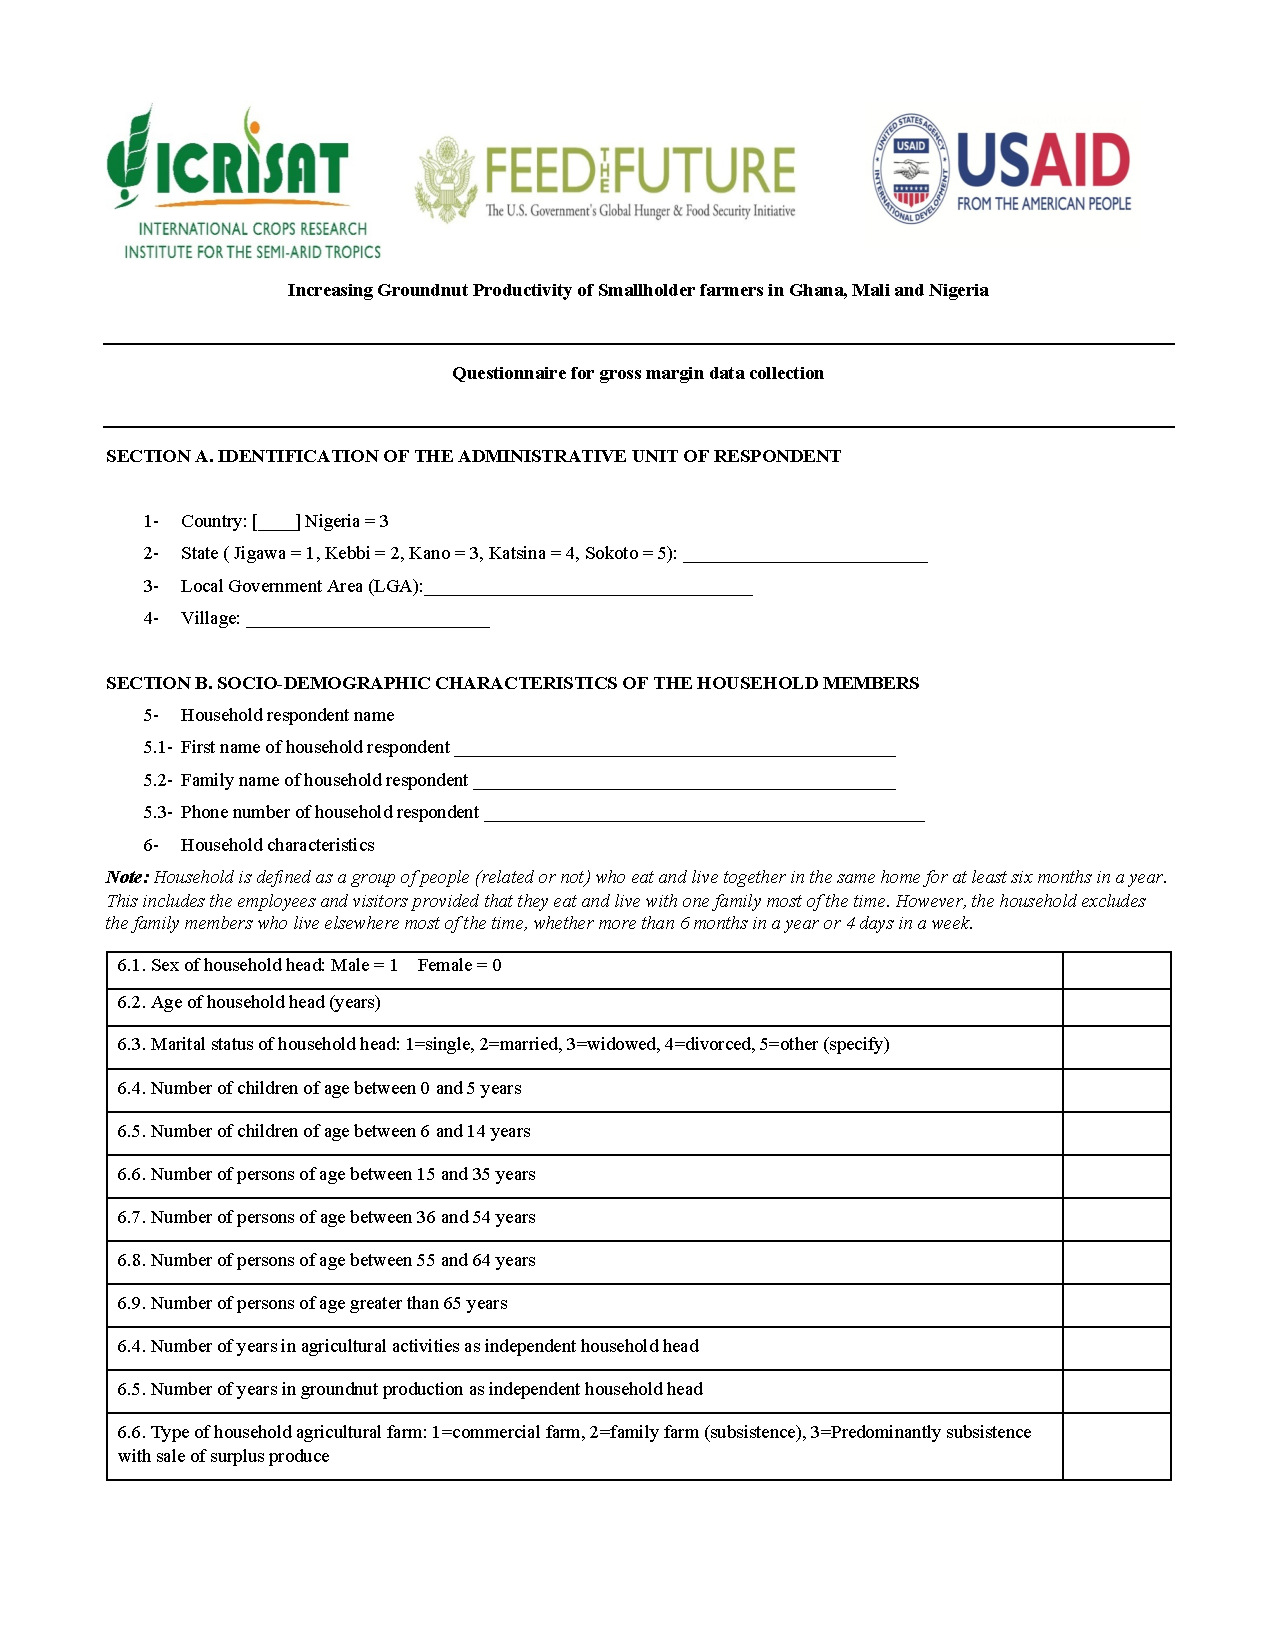
\includepdf[pages=-, pagecommand={}]{Questionnaire.pdf}

\end{document}
